\documentclass[a4paper,12pt]{article} 


\usepackage[T2A]{fontenc}			
\usepackage[utf8]{inputenc}			
\usepackage[english,russian]{babel}	

\usepackage{graphicx, scalerel}    
\usepackage{wrapfig}               
\usepackage[14pt]{extsizes}        
\usepackage[warn]{mathtext}       
\usepackage{indentfirst}      
\usepackage[margin = 25mm]{geometry}
\usepackage[table,xcdraw]{xcolor} 
\usepackage{amsmath,amsfonts,amssymb,amsthm,mathtools}
\usepackage{wasysym}                
\usepackage{upgreek}                
\usepackage{caption}
\usepackage{multirow}
\captionsetup{labelsep=period}
\usepackage[font=small,labelfont=bf]{caption}
\usepackage{gensymb}
\usepackage[unicode, pdftex]{hyperref}
\usepackage{tikz}
\usetikzlibrary{positioning}
\usepackage{fancyhdr}
\pagestyle{fancy}
\setlength\fboxsep{3pt} % Отступ рамки \fbox{} от рисунка
\setlength\fboxrule{1pt} % Толщина линий рамки \fbox{}
\newcommand{\tocsection}[1]{\section*{#1} \addcontentsline{toc}{section}{#1}}
\newcommand{\tocsubsection}[1]{\subsection*{#1} \addcontentsline{toc}{subsection}{#1}}
\renewcommand{\cftsecleader}{\cftdotfill{\cftdotsep}}

\def\fillandplacepagenumber{%
	\par\pagestyle{empty}%
	\vbox to 0pt{\vss}\vfill
	\vbox to 0pt{\baselineskip0pt
		\hbox to\linewidth{\hss}%
		\baselineskip\footskip
		\hbox to\linewidth{%
			\hfil\thepage\hfil}\vss}}

\begin{document}
		\newcommand{\HRule}{\rule{\linewidth}{0.7mm}} % Defines a new command for the horizontal lines, change thickness here

\begin{center}
	\large\textbf{Московский Физико-Технический Институт}\\
	\large\textbf{(государственный университет)}
	
	\vfill
	

	
	\Large Вычислительная математика
	%----------------------------------------------------------------------------------------
	%	TITLE SECTION
	%----------------------------------------------------------------------------------------
	
	\HRule
	\\[0.4cm]
	{ \huge \bfseries Лабораторная работа №9}
	\\[0.4cm] % Title of your document
	\HRule
	\\[0.5cm]
	
	\ \\
	\textbf{\large Автор:} \\	
	\large Овсянников Михаил Б01-008\\
	\vfill
	\hspace*{-0.8 cm}
\includegraphics[width=100 pt]{./Include/frkt_logo.pdf}\\
	\large Долгопрудный, 2023
\end{center}

\thispagestyle{empty}

\newpage
\setcounter{page}{2}
\fancyfoot[c]{\thepage}
\fancyhead[L] {Лабораторная работа №9}
\fancyhead[R]{}

		\tableofcontents
		\newpage
		
		\tocsection{Цель}
		Реализовать явные методы решения систем обыкновенных дифференциальных уравнений. Использовать методы Рунге-Кутты и многошаговые методы.  
		
		\tocsection{Теоретические сведения}
		
		\tocsubsection{Общая задача}
		Пусть нам дана система обыкновенных дифференциальных уравнений (ОДУ) с начальным условием:
		\begin{equation*}
			\begin{cases}
				y'(x) = f(x, y),\\
				y(x_0) = y_0.
			\end{cases}
		\end{equation*}
	
		Здесь $x$ предполагается одномерной независимой переменной, а $y$ -- многомерный вектор-решение.
		
		Требуется численно решить данную систему явными методами. В данной работе будут использоваться классический метод Рунге-Кутты 4 порядка и многошаговый метод Адамса 4 порядка.
		
		\tocsubsection{Описание классического метода Рунге-Кутты 4 порядка}
		Данный метод является многостадийным, следующее значение $y_{n+1}$ получается из предыдущего следующим образом:
		\begin{equation*}
			y_{n+1} = y_n + \frac{h}{6}(f_1 + 2f_2 + 2f_3 + f_4),
		\end{equation*}
		\noindent где $h$ -- шаг сетки и
		\begin{equation*}
		\begin{split}
			f_1 & = f(x_n, y_n), \\
			f_2 & = f(x_n + \frac{h}{2}, y_n + \frac{h}{2}f_1), \\
			f_3 & = f(x_n + \frac{h}{2}, y_n + \frac{h}{2}f_2), \\
			f_4 & = f(x_n + h, y_n + hf_3).
		\end{split}
		\end{equation*}
	
		Данный метод имеет 4 порядок точности, однако он является явным, поэтому могут возникнуть проблемы с его устойчивостью.
		
		\tocsubsection{Описание многошагового метода Адамса 4 порядка}
		Другим классом методов решения ОДУ и систем ОДУ являются многошаговые методы. Конкретно в этой работе рассматривается метод Адамса четвертого порядка. Выглядит он следующим образом:
		
		\small
		\begin{equation*}
			y_{n+1} = y_n + h\left(\frac{55}{24}f(x_n, y_n) - \frac{59}{24}f(x_{n-1}, y_{n-1}) + \frac{37}{24}f(x_{n-2}, y_{n-2}) - \frac{3}{8}f(x_{n-3}, y_{n-3})\right).
		\end{equation*}
	
		\normalsize
	
		То есть для подсчета новой точки мы используем не только последнюю, но и несколько других до нее. Конкретно здесь для подсчета новой точки мы используем информацию о четырех предыдущих.
		
		Возникает проблема при подсчете второй, третьей и четвертой точки -- мы не можем их посчитать данным методом. Выходом является подсчет этих точек другими методами, например, методами Рунге-Кутты, а дальше уже считаем методом Адамса.
		
		\tocsection{Непосредственно задание}
		
		\tocsubsection{Постановка задачи}
		
		В качестве упражнения была взята система \textbf{VIII.11.1} первой части сборника Аристовой, Лобанова и Завьяловой:
		\begin{equation*}
			\begin{cases}
				x' = A + x^2 y - (B + 1)x, \\
				y' = Bx - x^2 y, \\
				x(0) = y(0) = 1.
			\end{cases}
		\end{equation*}
	
		Здесь $A = 1$, $B \in [1, 5]$ -- параметры.
		
		Система является моделью Лефевра-Пригожина <<брюсселятор>>.
		
		Будем решать эту систему следующими методами:
		\begin{itemize}
			\item Классический метод Рунге-Кутты 4 порядка точности
			
			\item Многошаговый метод Адамса 4 порядка точности
		\end{itemize}
		
		\textit{В последнем методе}: нулевая точка задана, первую, вторую и третью посчитаем первым методом, а дальше считаем методом Адамса.
		
		
		\tocsubsection{Результаты}
		В качестве результатов покажем графики зависимостей $x(t)$ и $y(t)$, а также фазовые портреты.
		
		
		\newgeometry{left=1cm, right=2cm, bottom=0.3cm, top=1cm}

		\newpage
		\thispagestyle{empty}
		\begin{landscape}
		\textbf{1)} $A = 1$, $B = 1.5$	
		\begin{figure}[h!]
			\begin{minipage}[h]{0.55\linewidth}
				\center{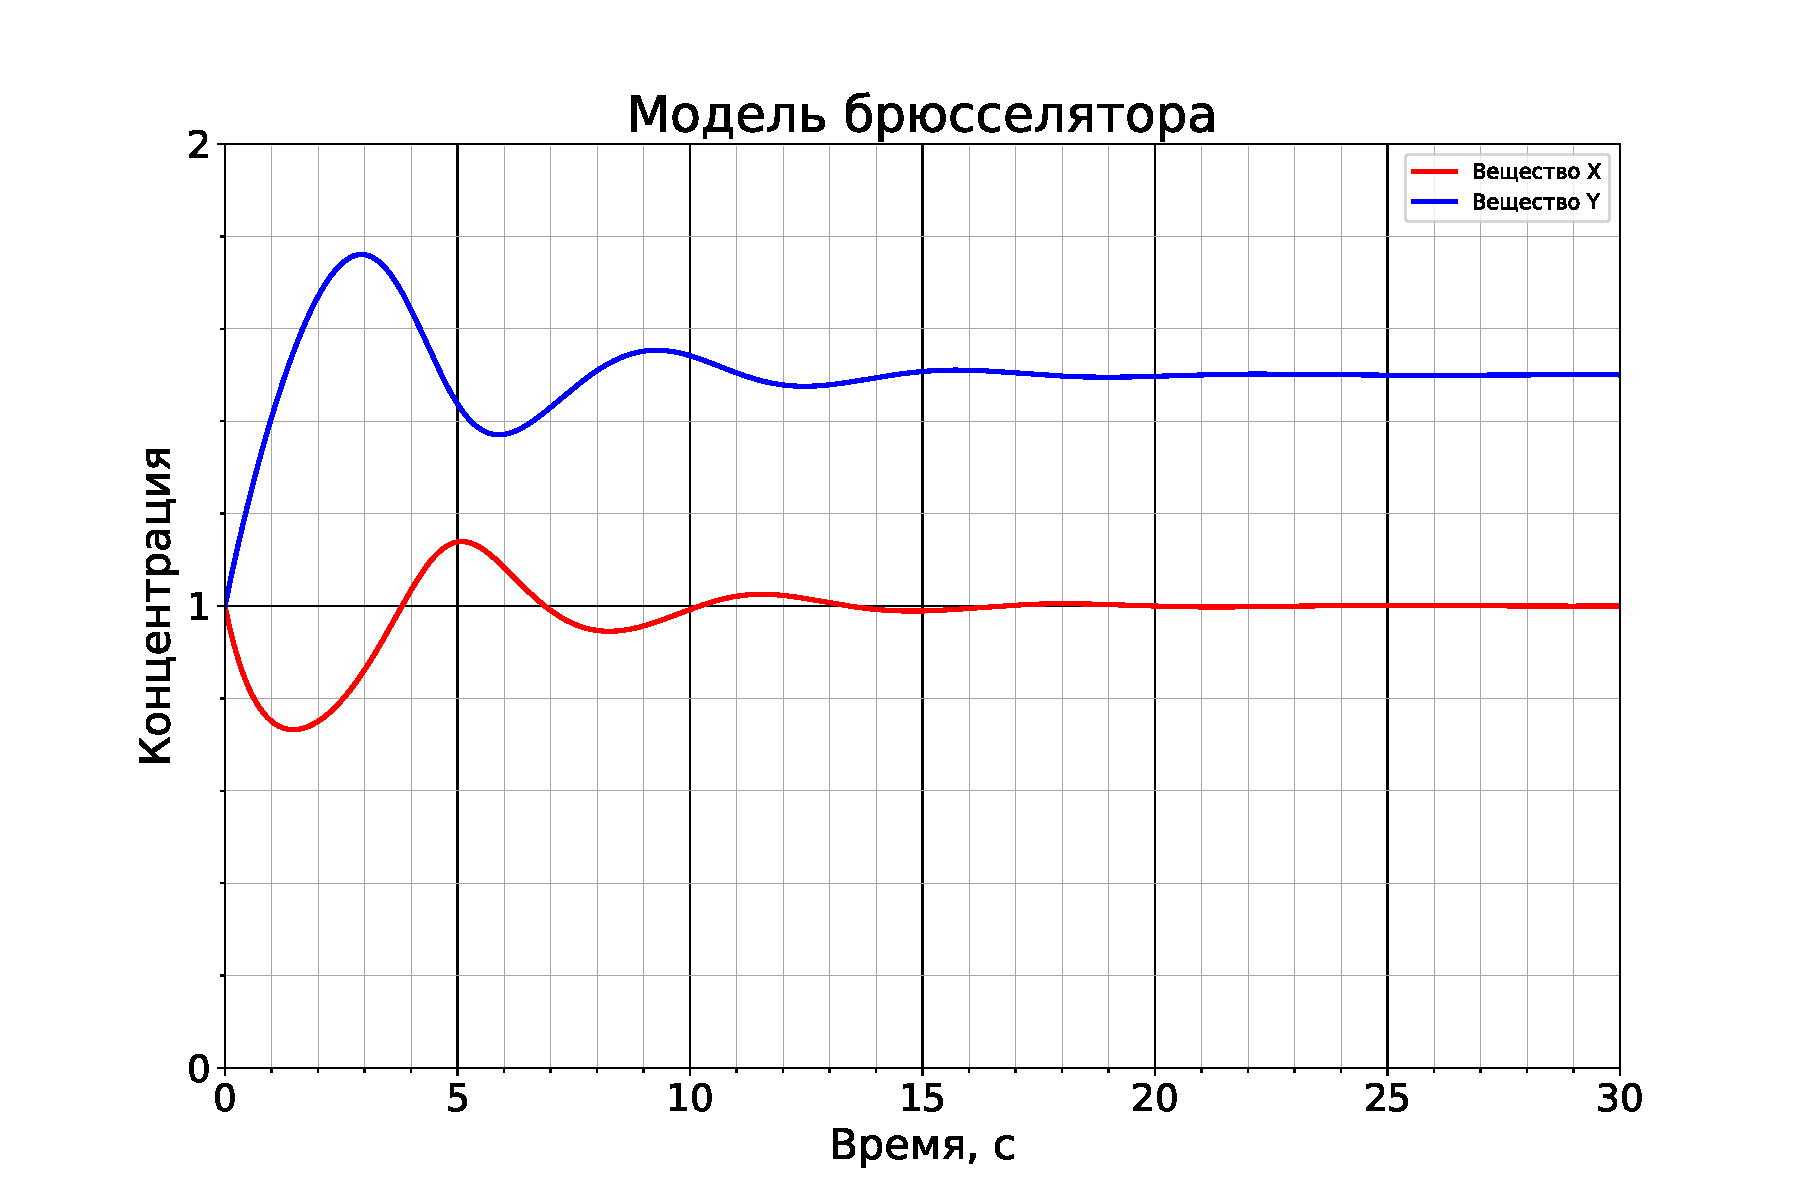
\includegraphics[width=1.2\linewidth]{Pictures/RungeKutta_B_1.5_conc}}
			\end{minipage}
			\hfill
			\begin{minipage}[h]{0.55\linewidth}
				\center{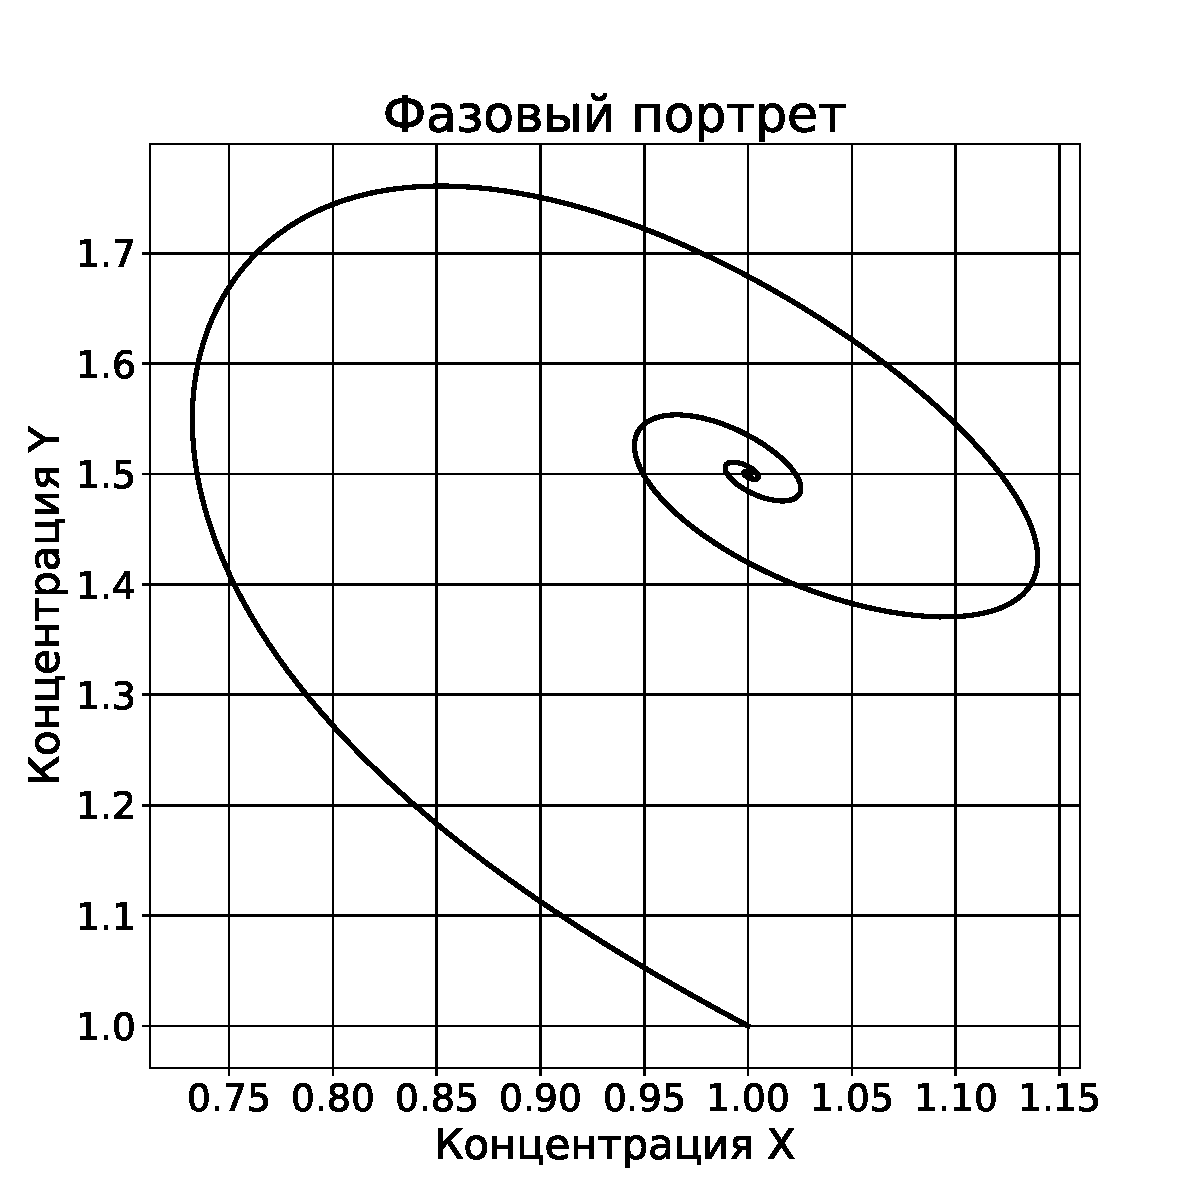
\includegraphics[width=0.8\linewidth]{Pictures/RungeKutta_B_1.5_phase}}
			\end{minipage}
			\caption{Решение методом Рунге-Кутты 4 порядка}
		\end{figure}
		\fillandplacepagenumber
		\end{landscape}
	
	
		\newpage
		\thispagestyle{empty}
		\begin{landscape}
			\begin{figure}[h!]
				\begin{minipage}[h]{0.55\linewidth}
					\center{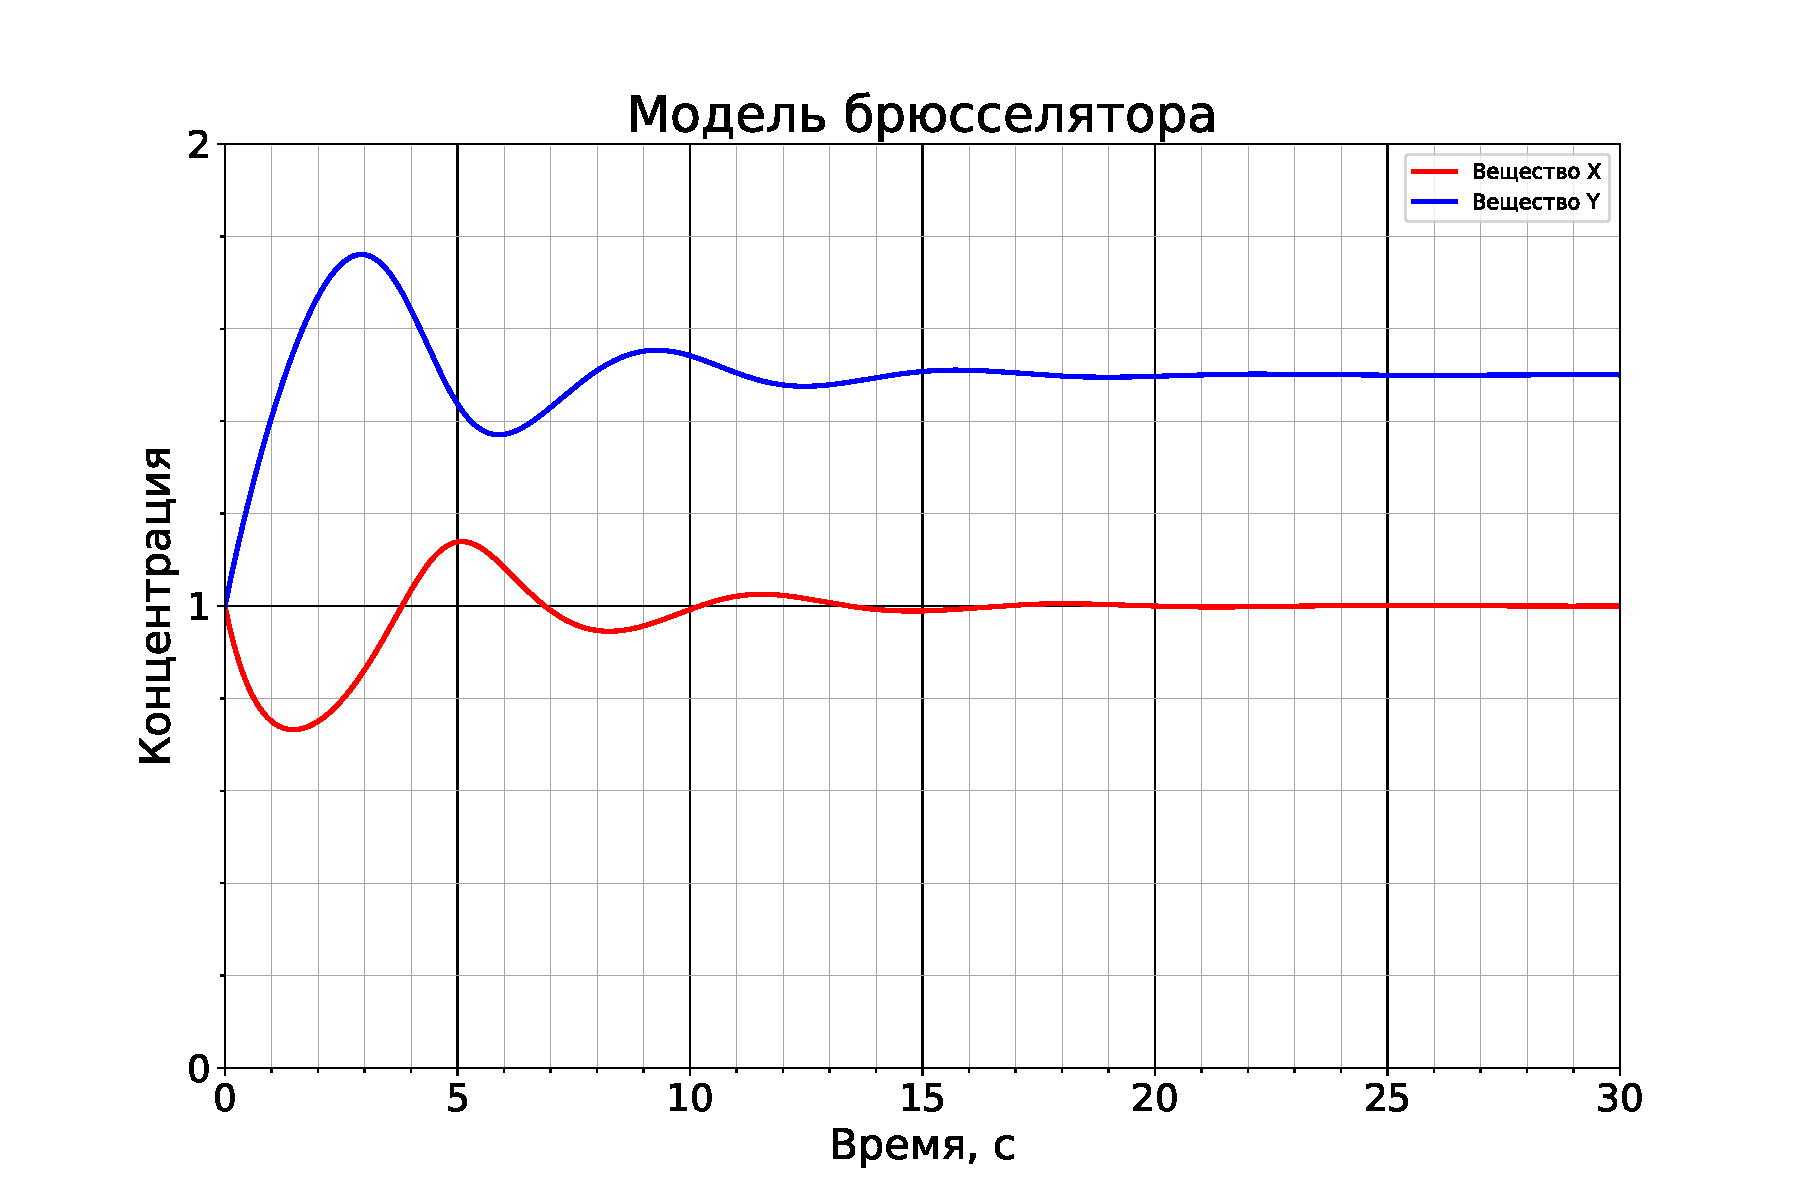
\includegraphics[width=1.2\linewidth]{Pictures/Adams_B_1.5_conc}}
				\end{minipage}
				\hfill
				\begin{minipage}[h]{0.55\linewidth}
					\center{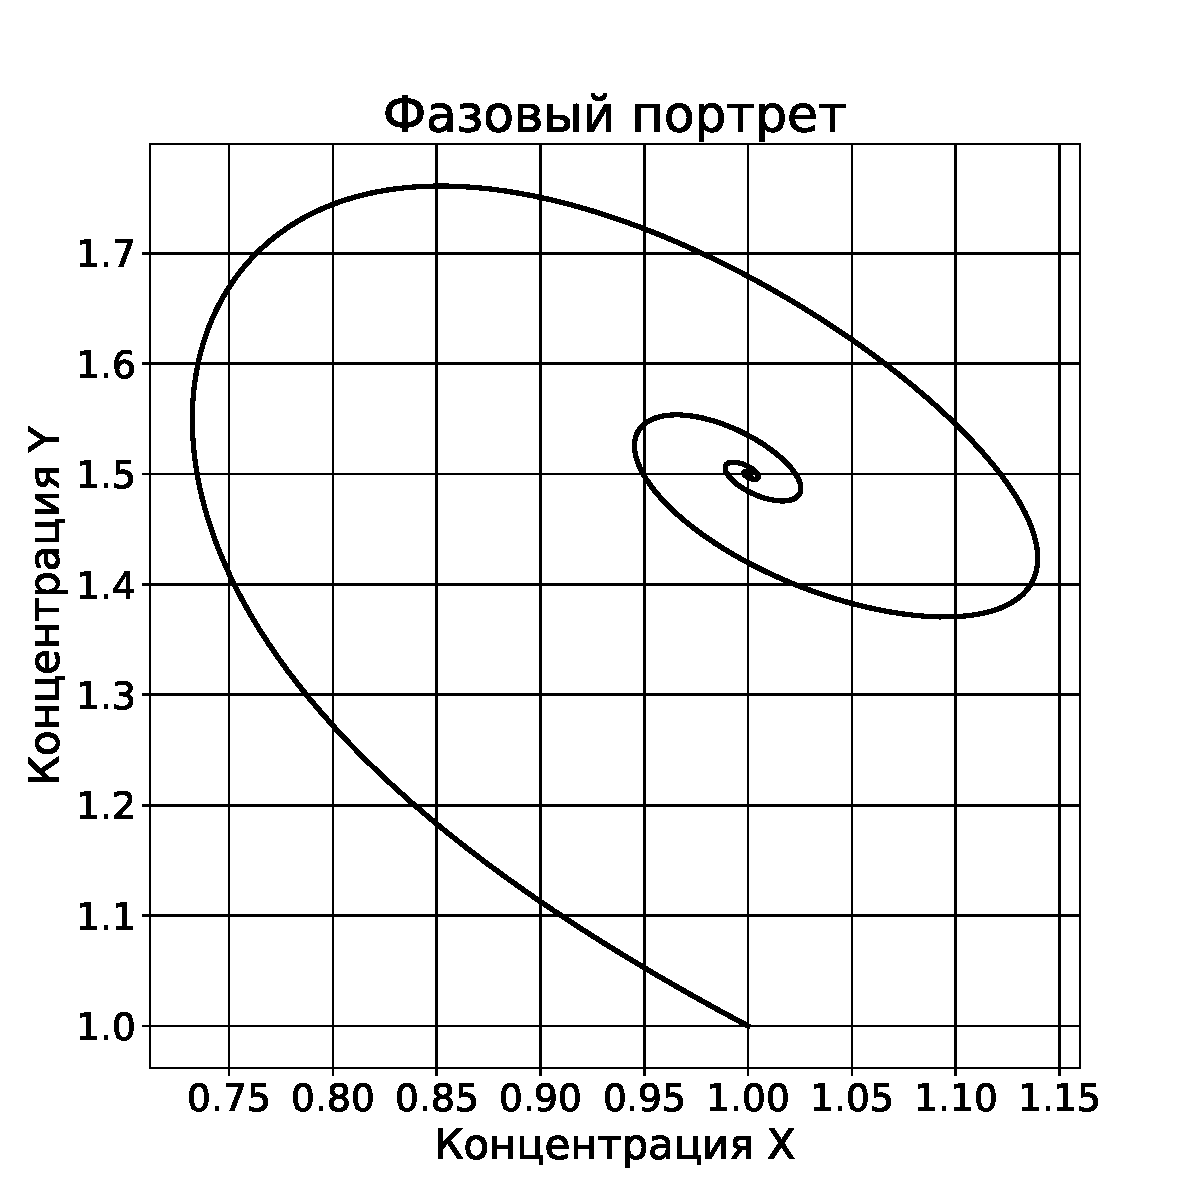
\includegraphics[width=0.8\linewidth]{Pictures/Adams_B_1.5_phase}}
				\end{minipage}
				\caption{Решение методом Адамса 4 порядка}
			\end{figure}
			\fillandplacepagenumber
		\end{landscape}
	
	
		
		\newpage
		\thispagestyle{empty}
		\begin{landscape}
			\textbf{2)} $A = 1$, $B = 2$	
			\begin{figure}[h!]
				\begin{minipage}[h]{0.55\linewidth}
					\center{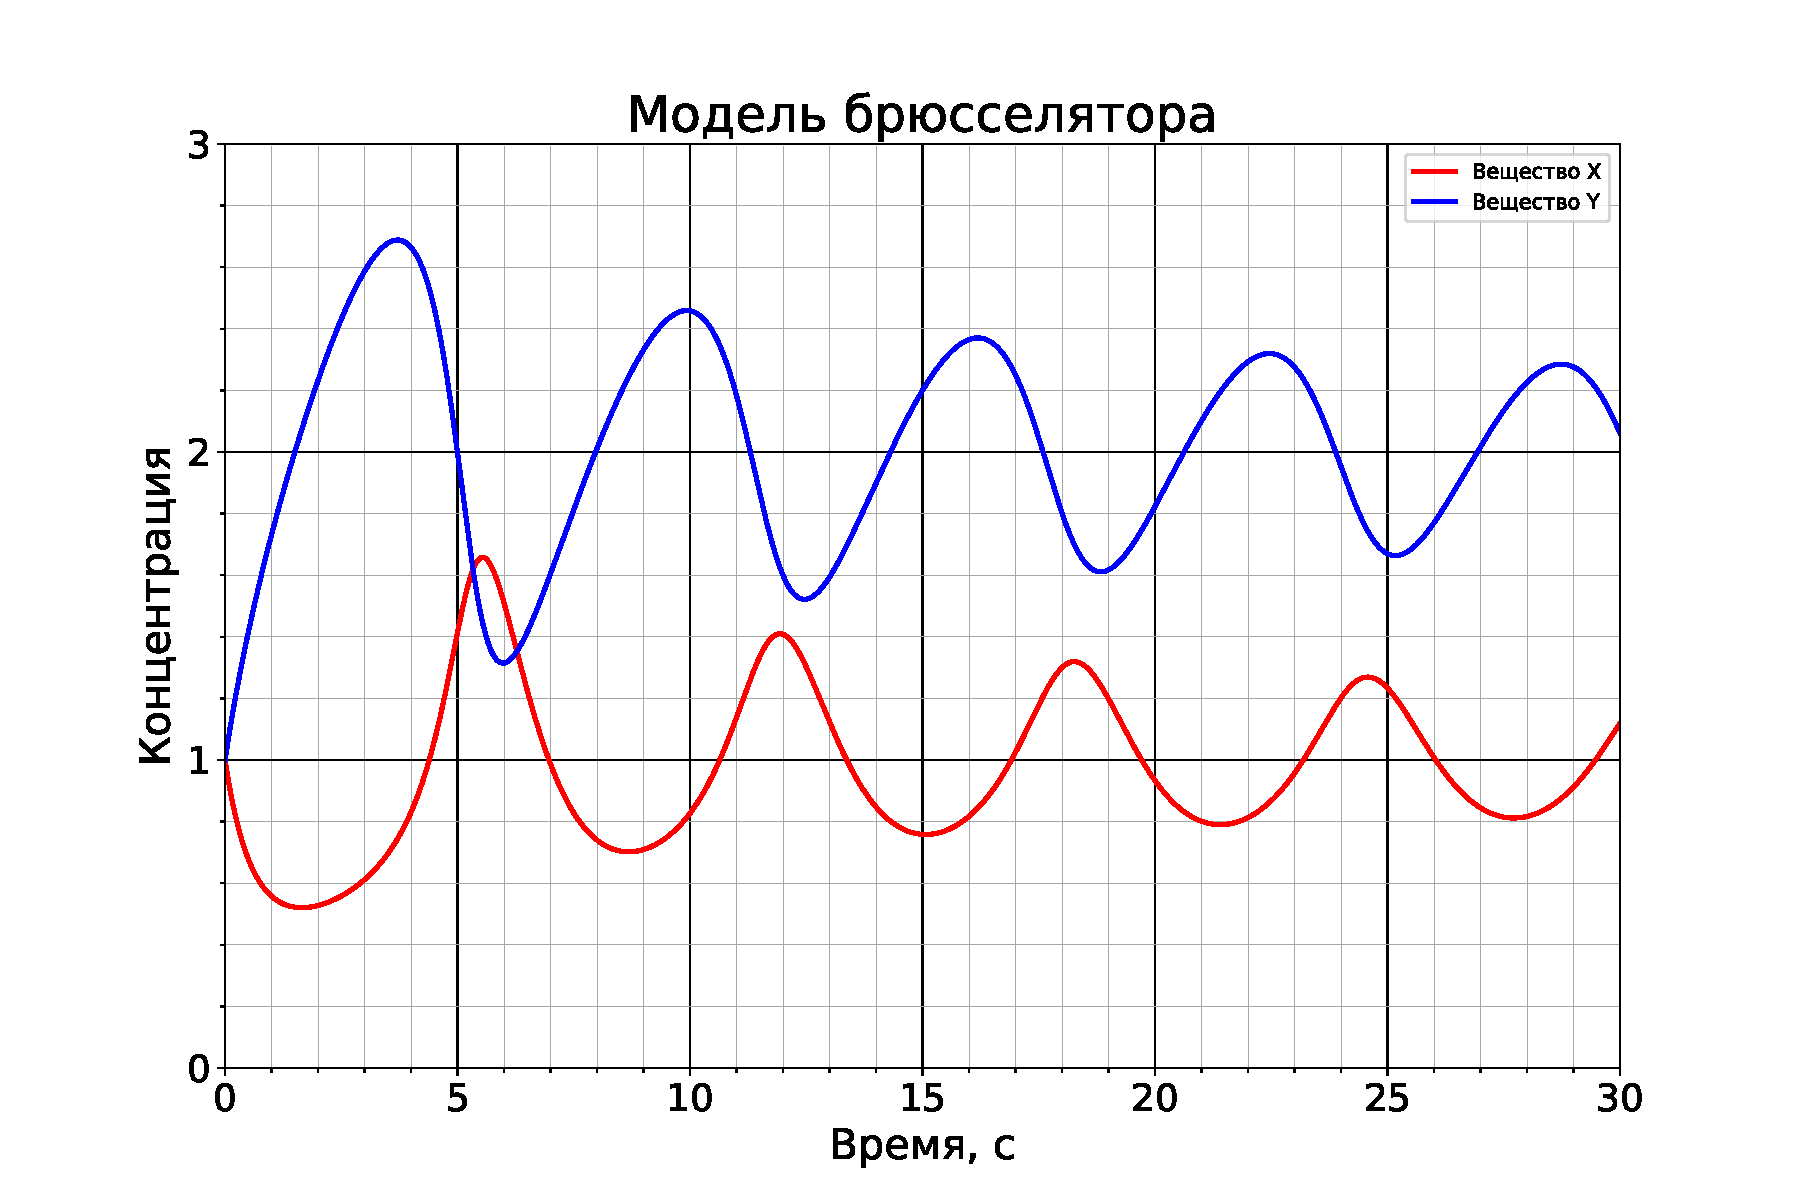
\includegraphics[width=1.2\linewidth]{Pictures/RungeKutta_B_2.0_conc}}
				\end{minipage}
				\hfill
				\begin{minipage}[h]{0.55\linewidth}
					\center{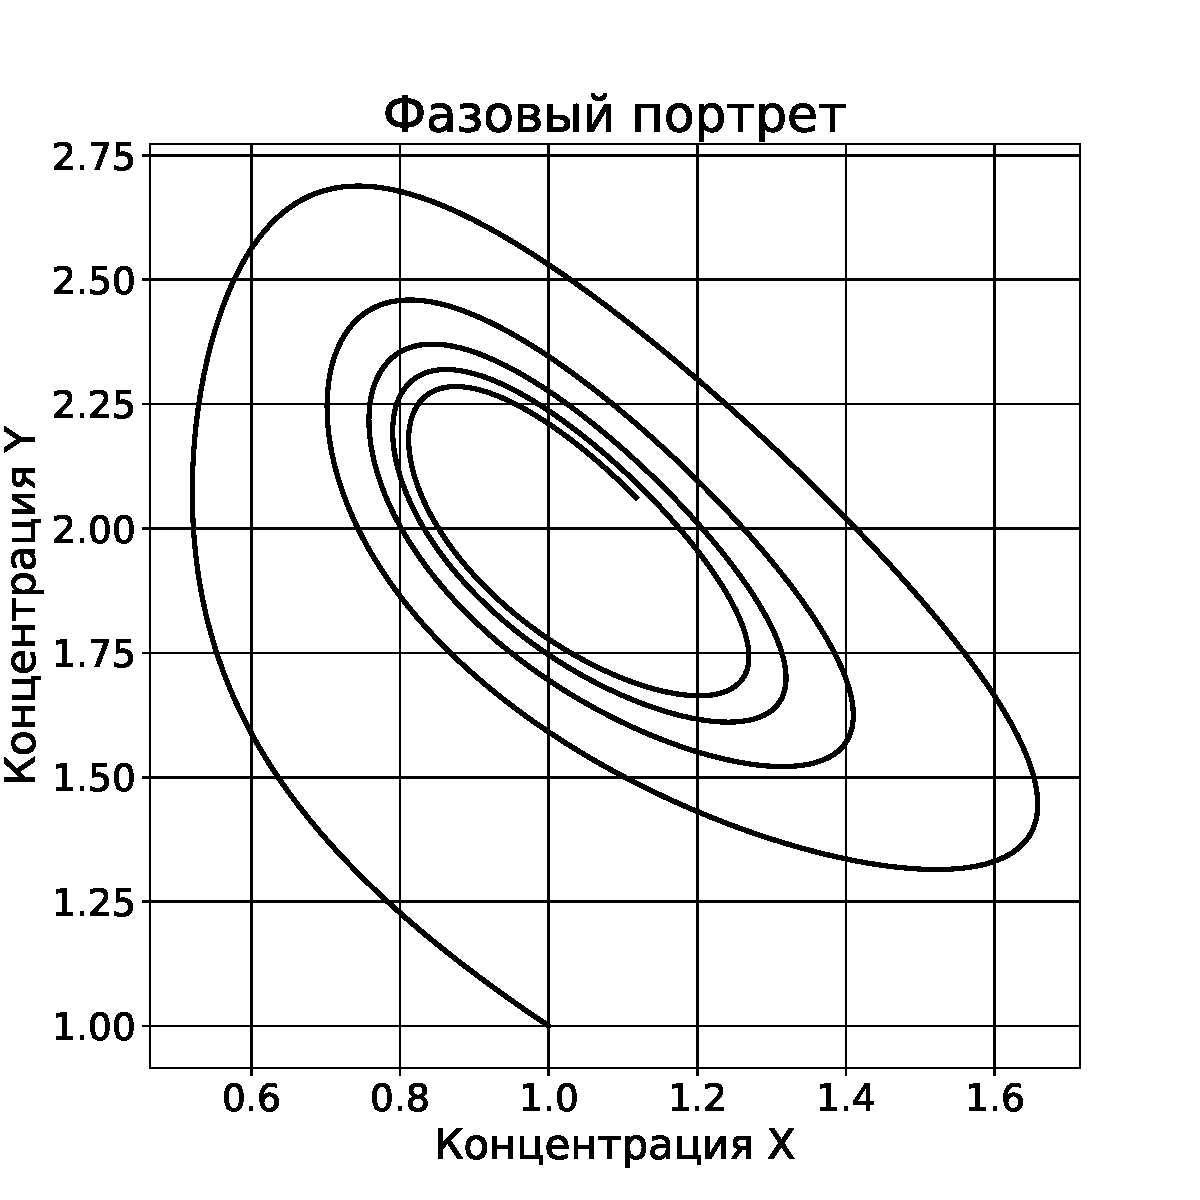
\includegraphics[width=0.8\linewidth]{Pictures/RungeKutta_B_2.0_phase}}
				\end{minipage}
				\caption{Решение методом Рунге-Кутты 4 порядка}
			\end{figure}
			\fillandplacepagenumber
		\end{landscape}
		
		
		\newpage
		\thispagestyle{empty}
		\begin{landscape}
			\begin{figure}[h!]
				\begin{minipage}[h]{0.55\linewidth}
					\center{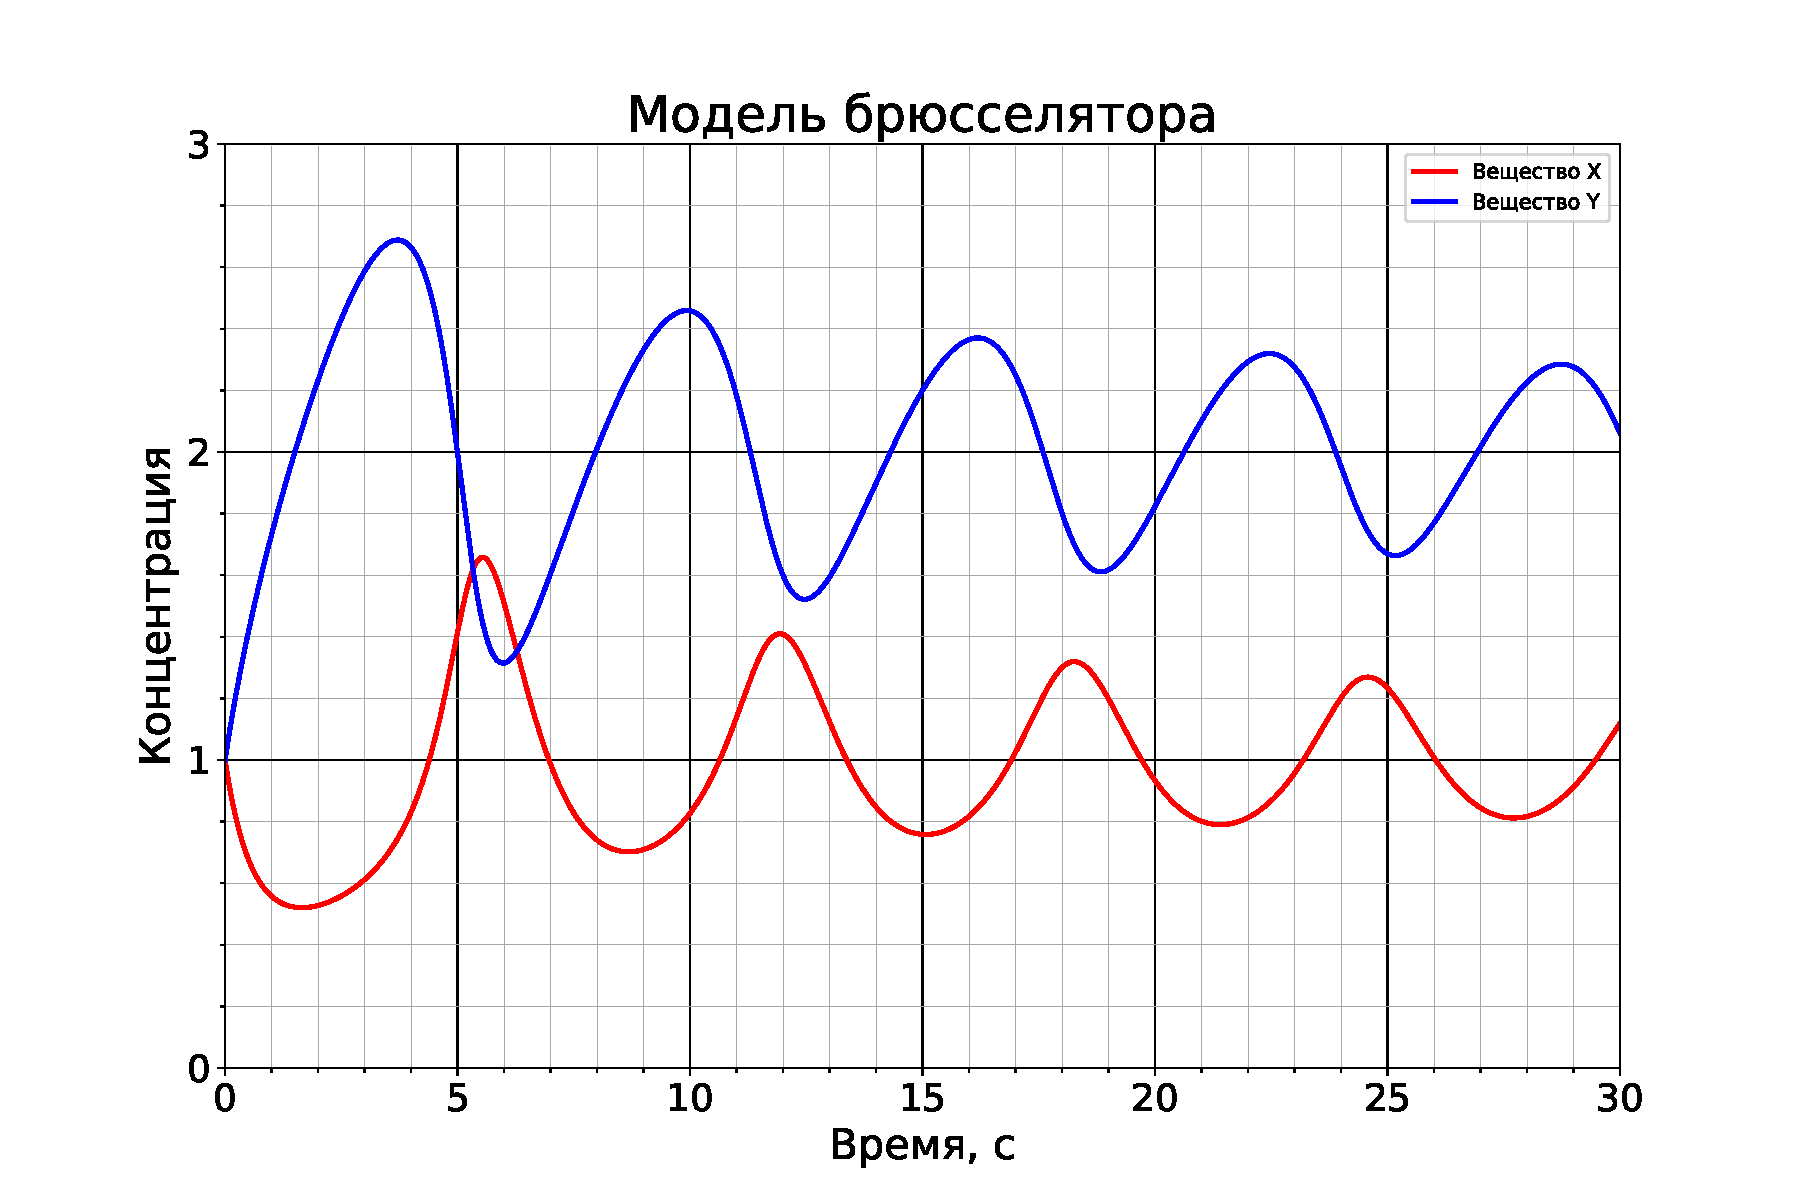
\includegraphics[width=1.2\linewidth]{Pictures/Adams_B_2.0_conc}}
				\end{minipage}
				\hfill
				\begin{minipage}[h]{0.55\linewidth}
					\center{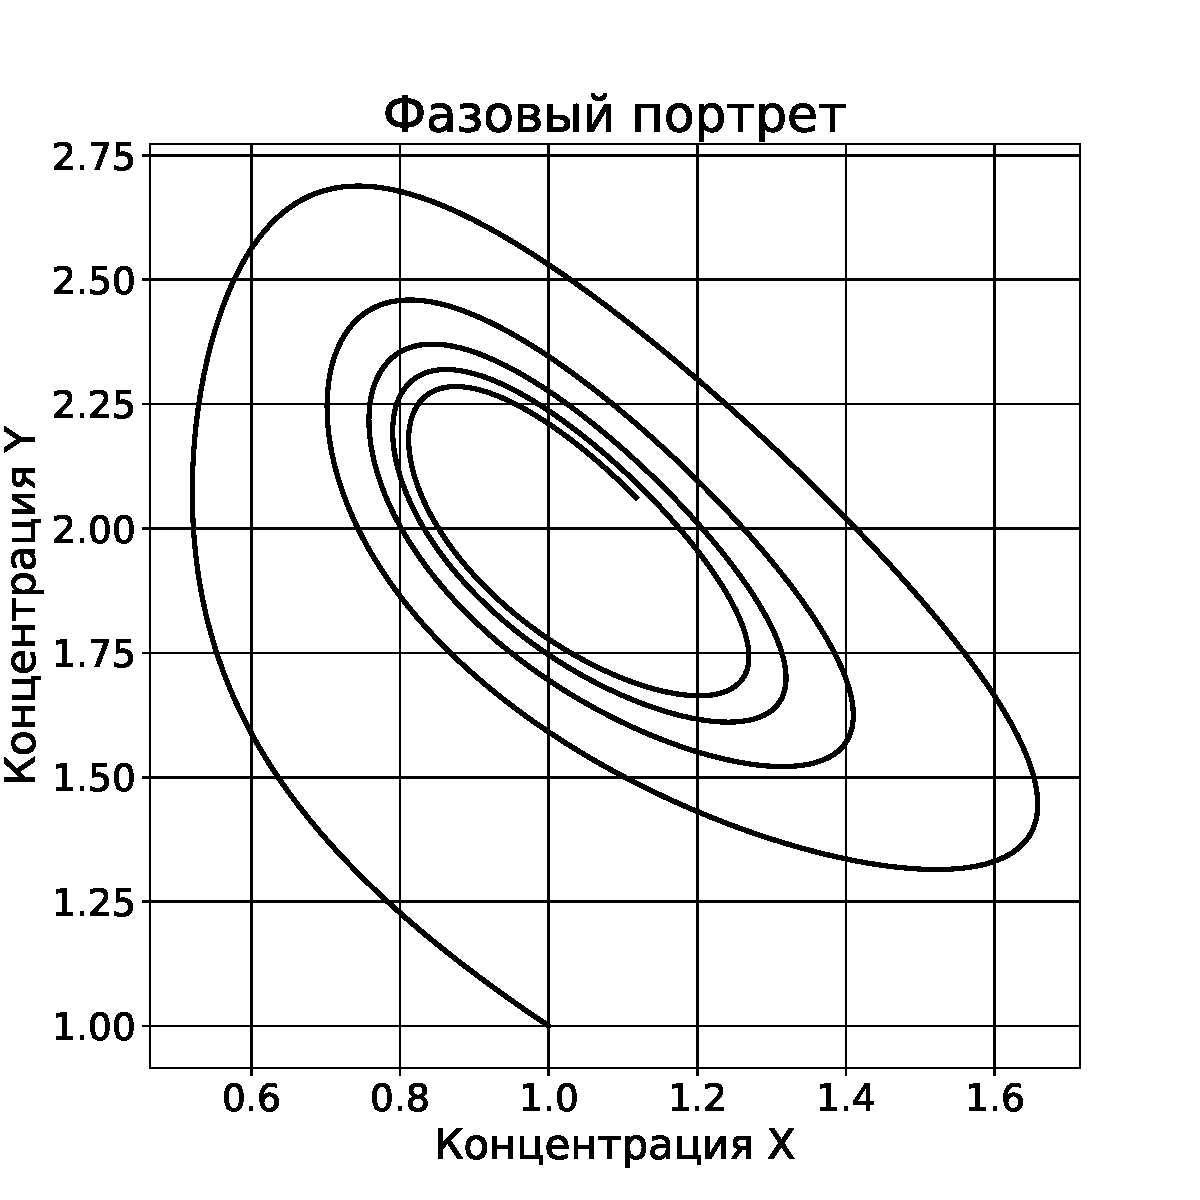
\includegraphics[width=0.8\linewidth]{Pictures/Adams_B_2.0_phase}}
				\end{minipage}
				\caption{Решение методом Адамса 4 порядка}
			\end{figure}
			\fillandplacepagenumber
		\end{landscape}
	
	
		\newpage
		\thispagestyle{empty}
		\begin{landscape}
			\textbf{3)} $A = 1$, $B = 3$	
			\begin{figure}[h!]
				\begin{minipage}[h]{0.55\linewidth}
					\center{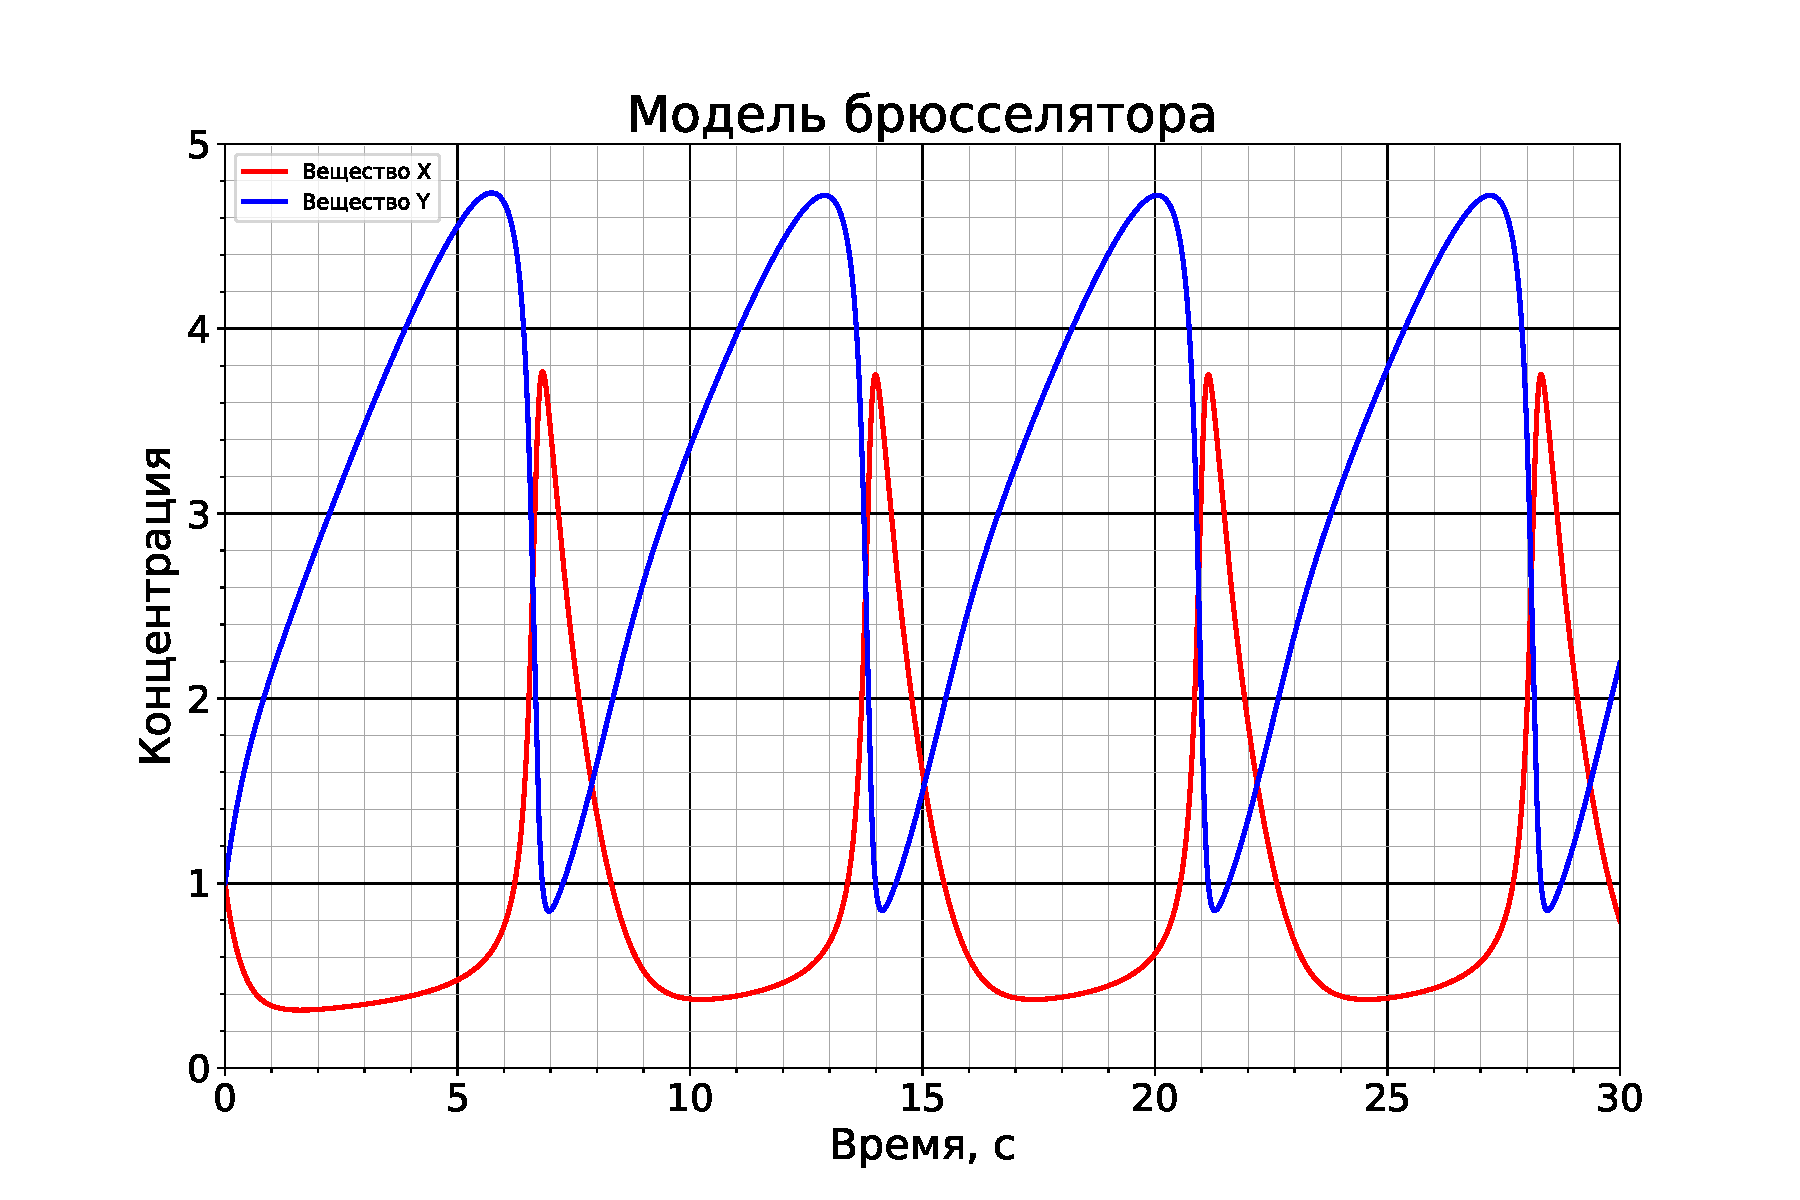
\includegraphics[width=1.2\linewidth]{Pictures/RungeKutta_B_3.0_conc}}
				\end{minipage}
				\hfill
				\begin{minipage}[h]{0.55\linewidth}
					\center{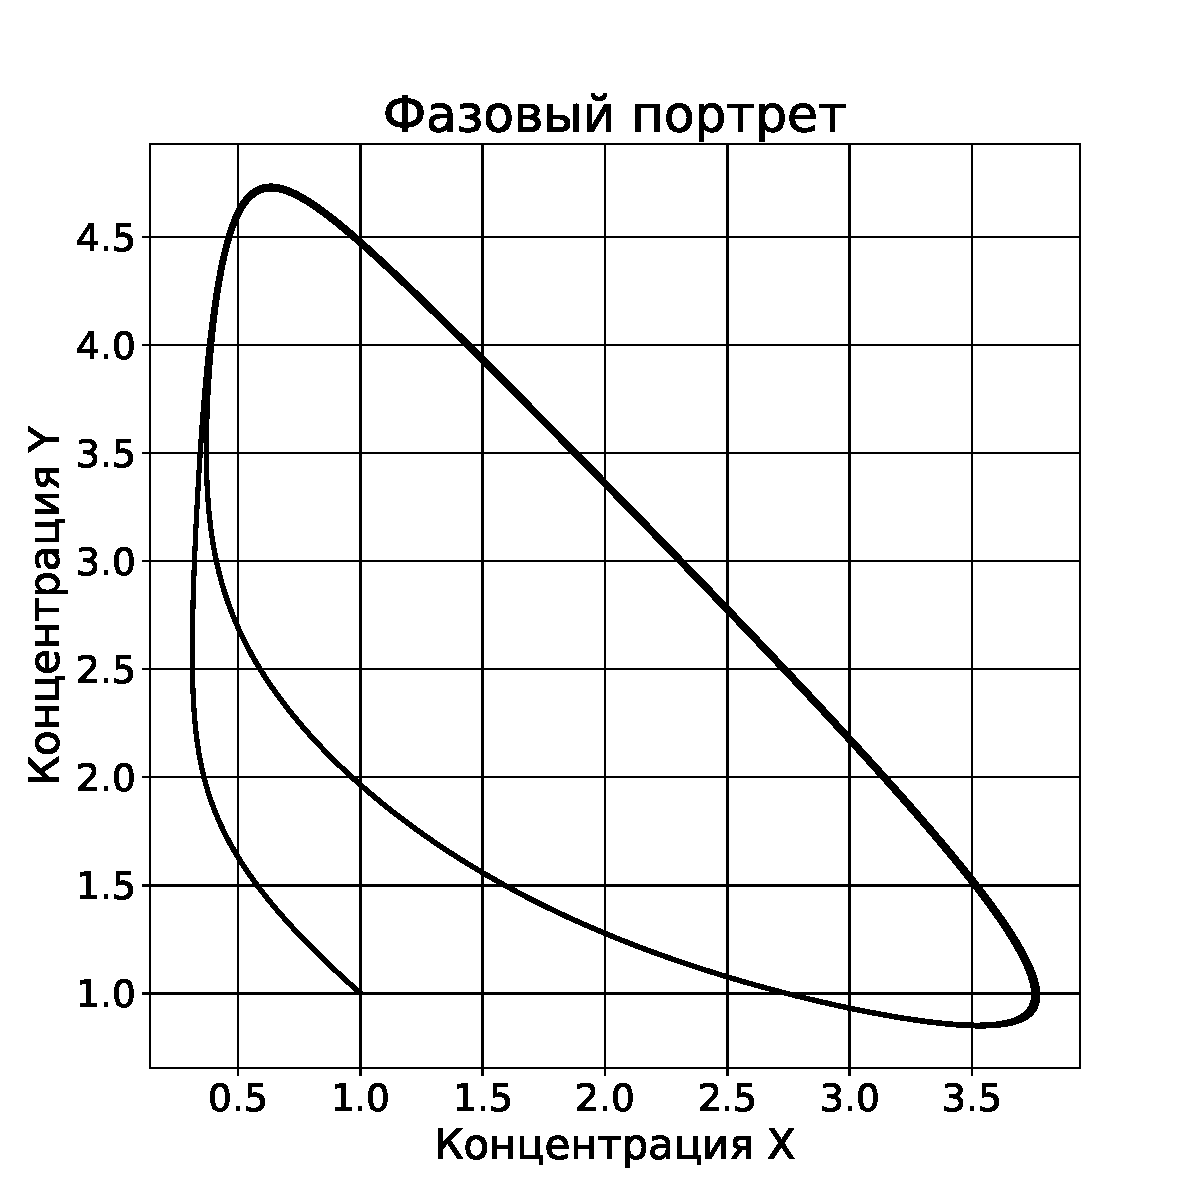
\includegraphics[width=0.8\linewidth]{Pictures/RungeKutta_B_3.0_phase}}
				\end{minipage}
				\caption{Решение методом Рунге-Кутты 4 порядка}
			\end{figure}
			\fillandplacepagenumber
		\end{landscape}
		
		
		\newpage
		\thispagestyle{empty}
		\begin{landscape}
			\begin{figure}[h!]
				\begin{minipage}[h]{0.55\linewidth}
					\center{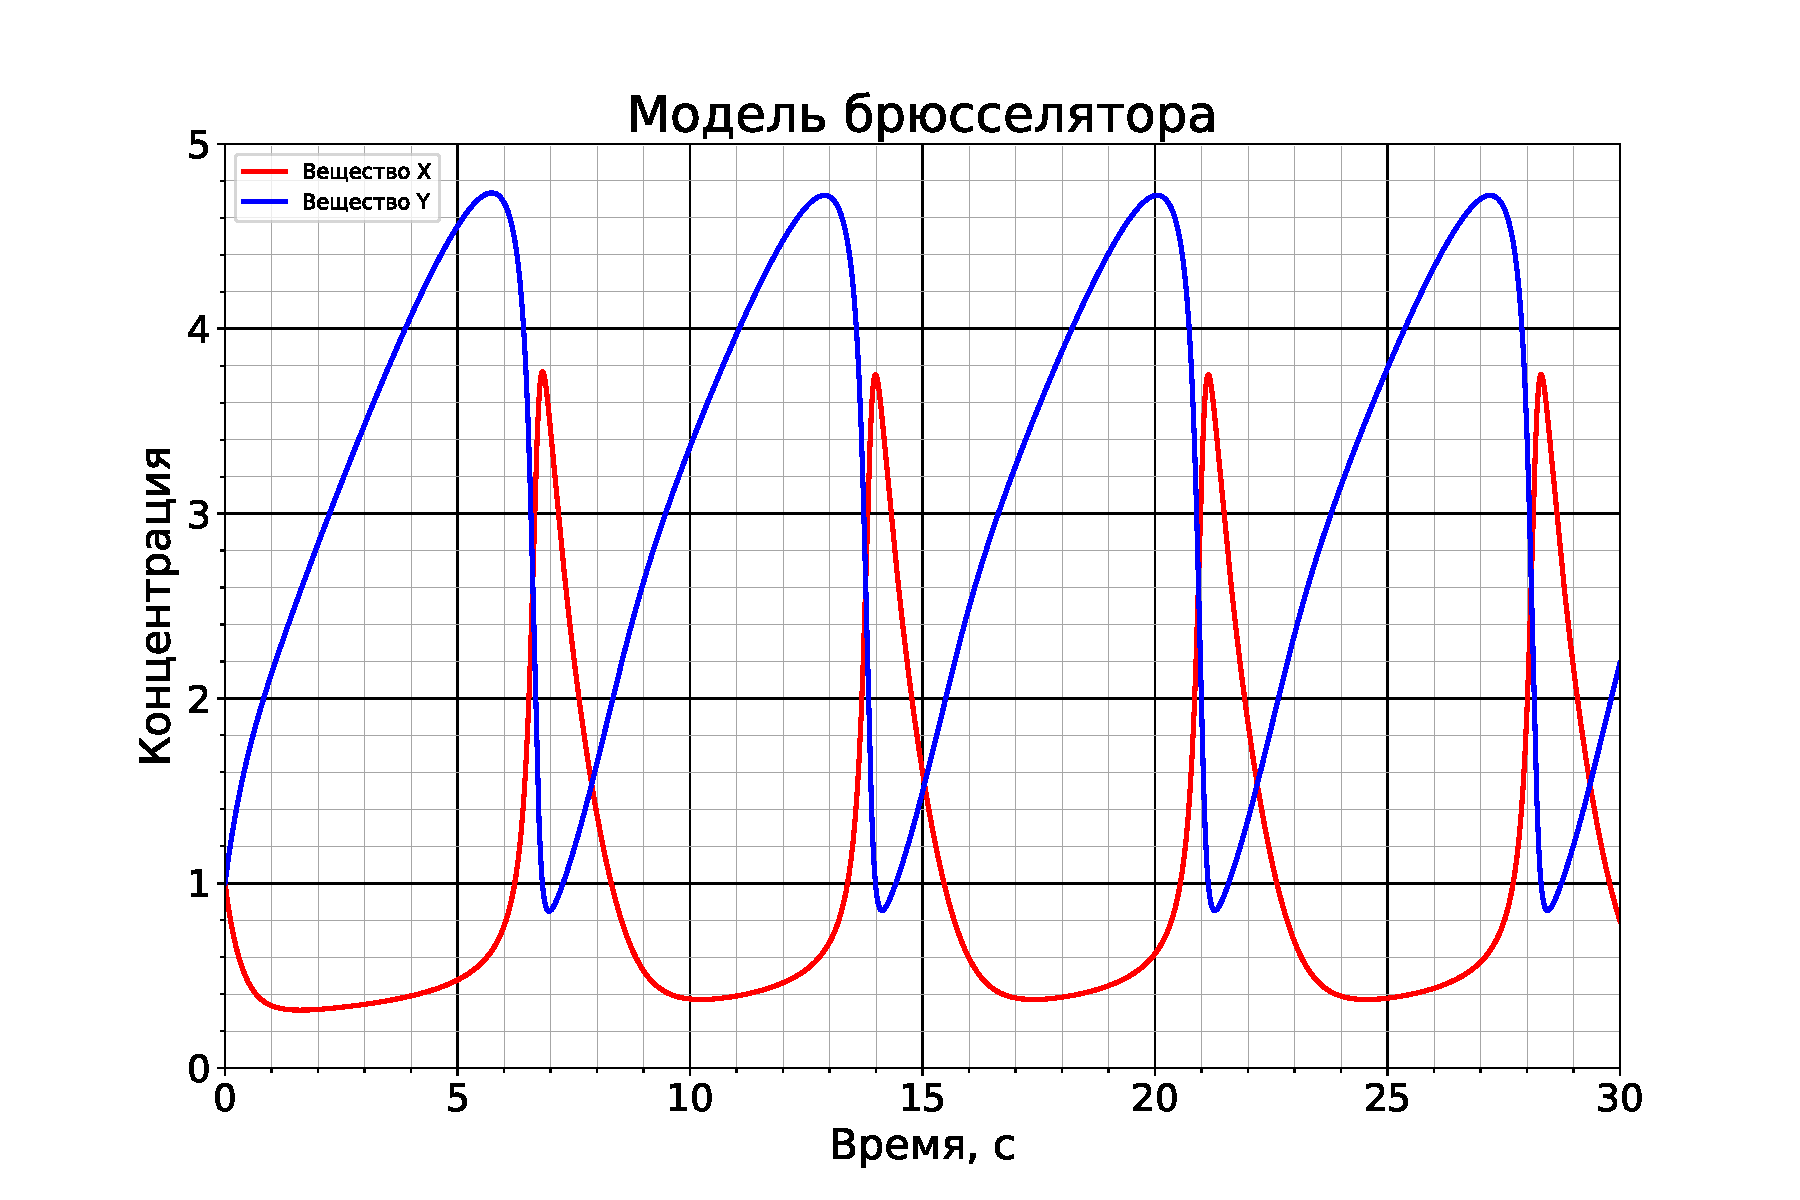
\includegraphics[width=1.2\linewidth]{Pictures/Adams_B_3.0_conc}}
				\end{minipage}
				\hfill
				\begin{minipage}[h]{0.55\linewidth}
					\center{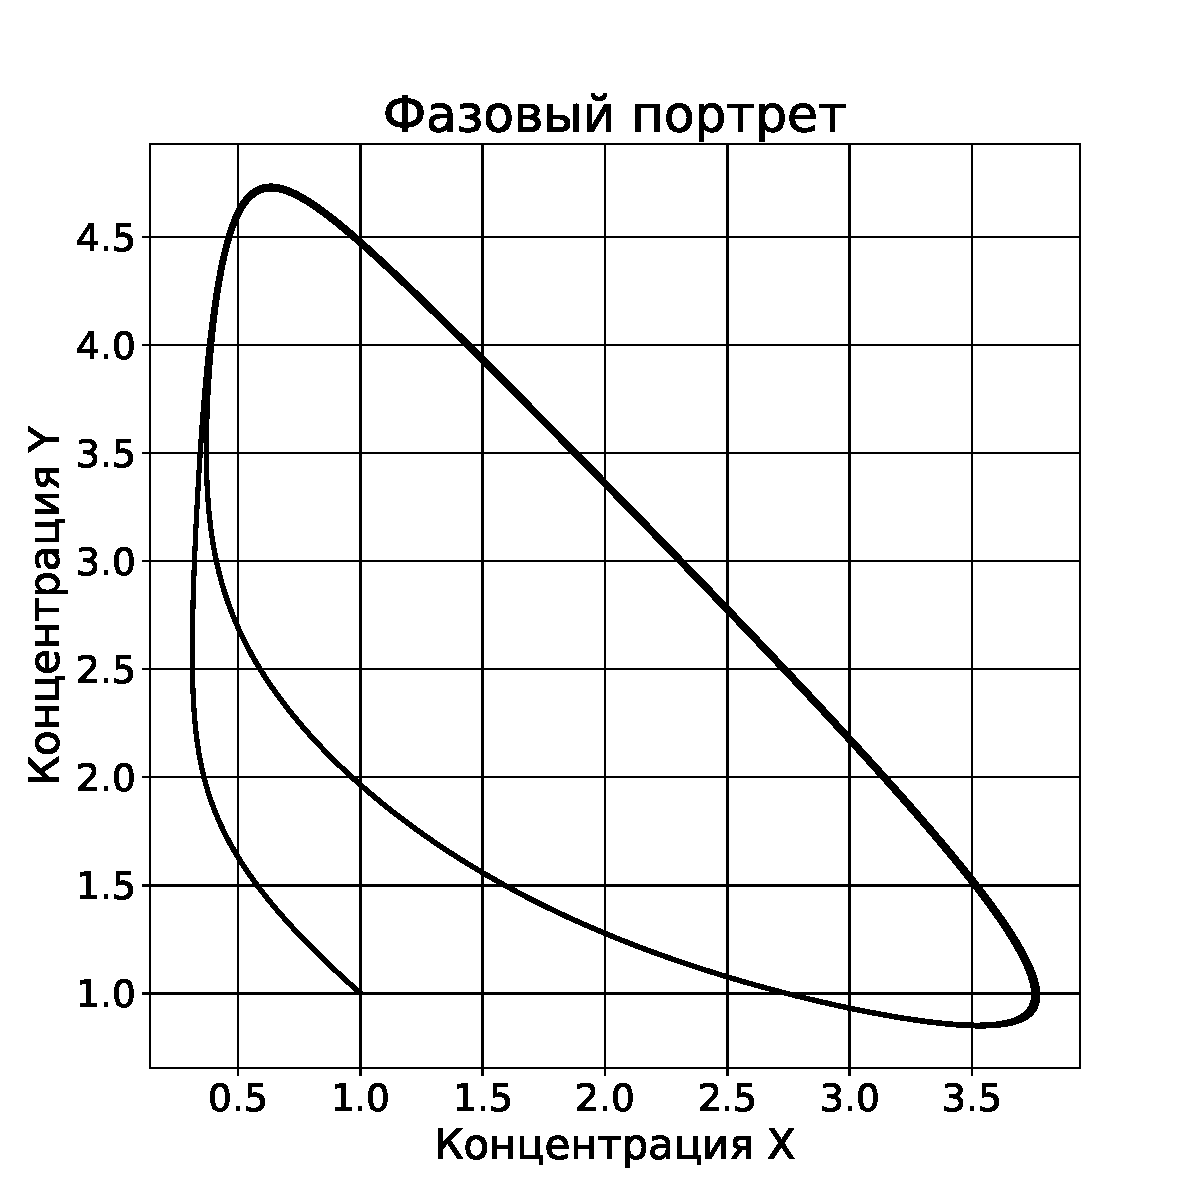
\includegraphics[width=0.8\linewidth]{Pictures/Adams_B_3.0_phase}}
				\end{minipage}
				\caption{Решение методом Адамса 4 порядка}
			\end{figure}
			\fillandplacepagenumber
		\end{landscape}
	
	
		\newpage
		\thispagestyle{empty}
		\begin{landscape}
			\textbf{4)} $A = 1$, $B = 4$	
			\begin{figure}[h!]
				\begin{minipage}[h]{0.55\linewidth}
					\center{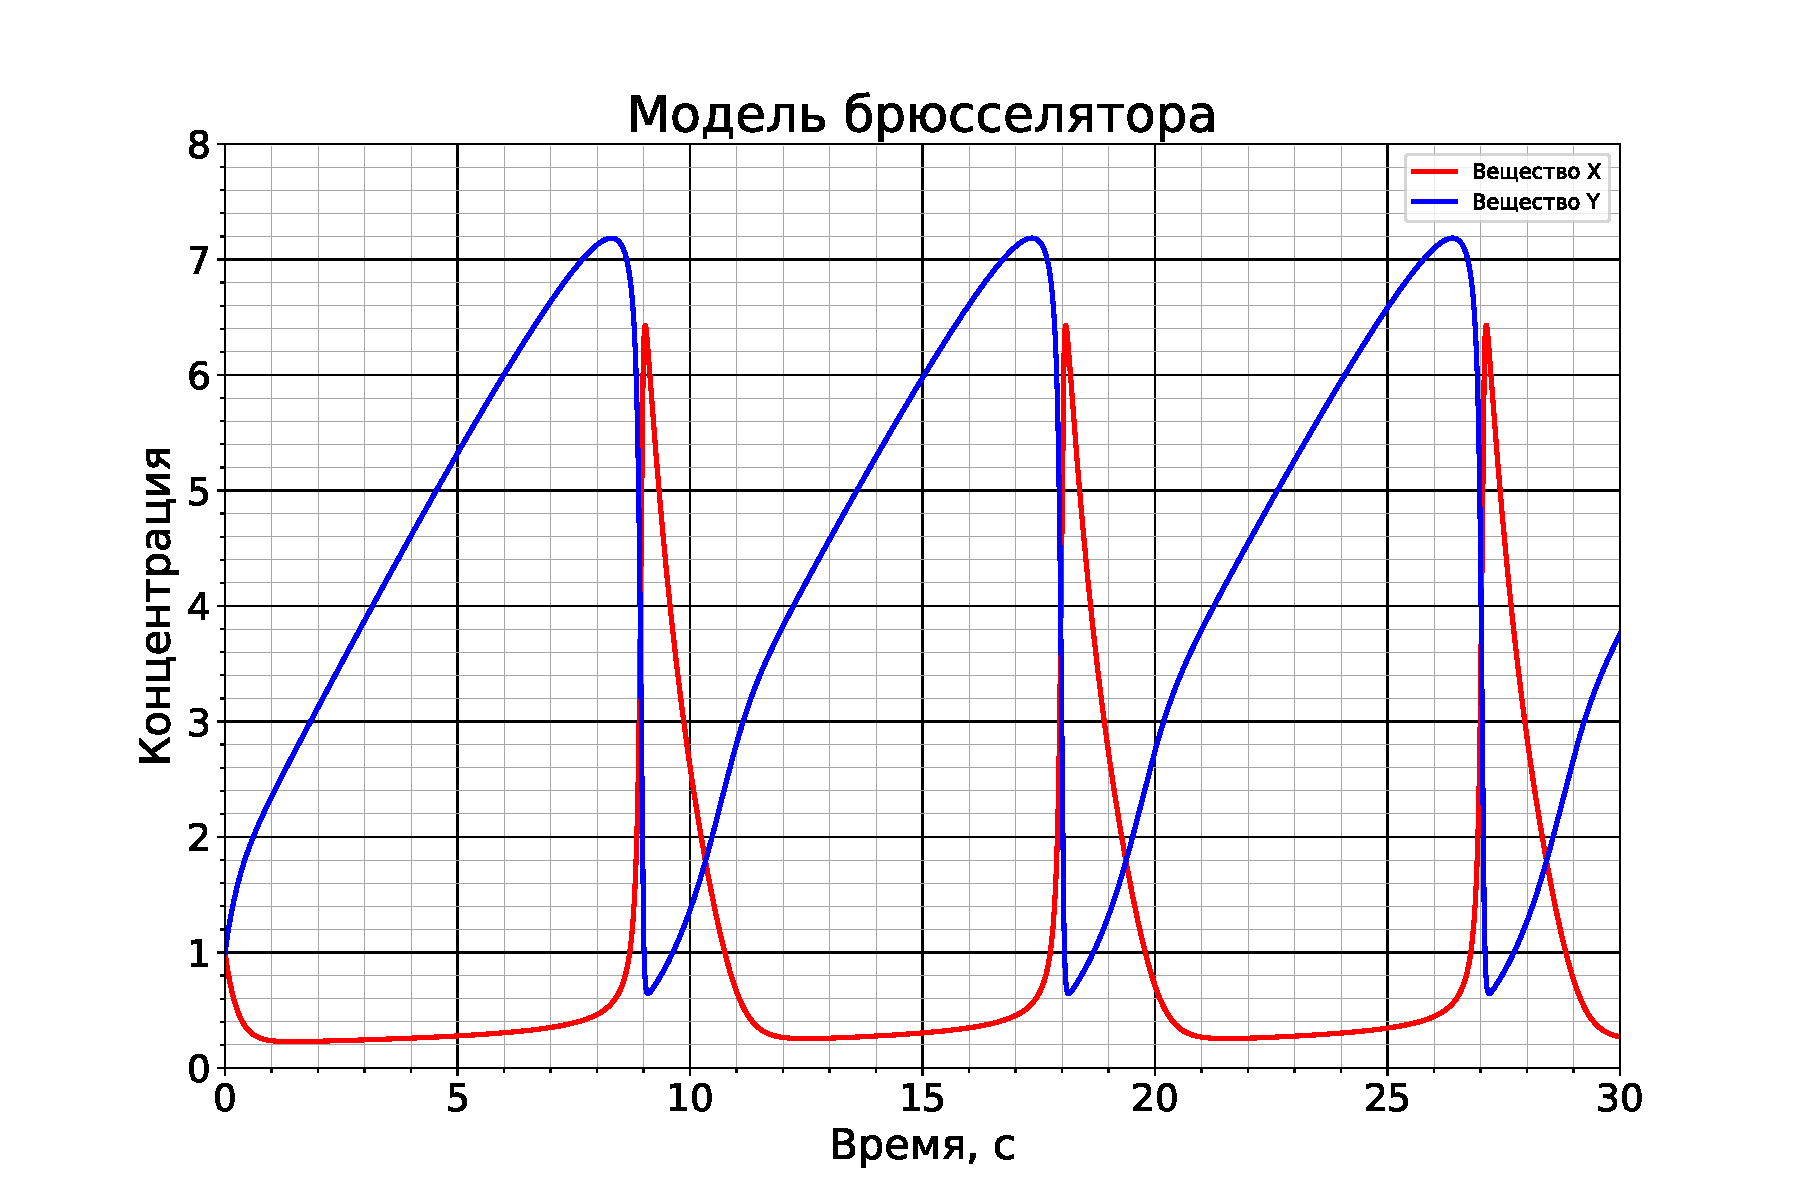
\includegraphics[width=1.2\linewidth]{Pictures/RungeKutta_B_4.0_conc}}
				\end{minipage}
				\hfill
				\begin{minipage}[h]{0.55\linewidth}
					\center{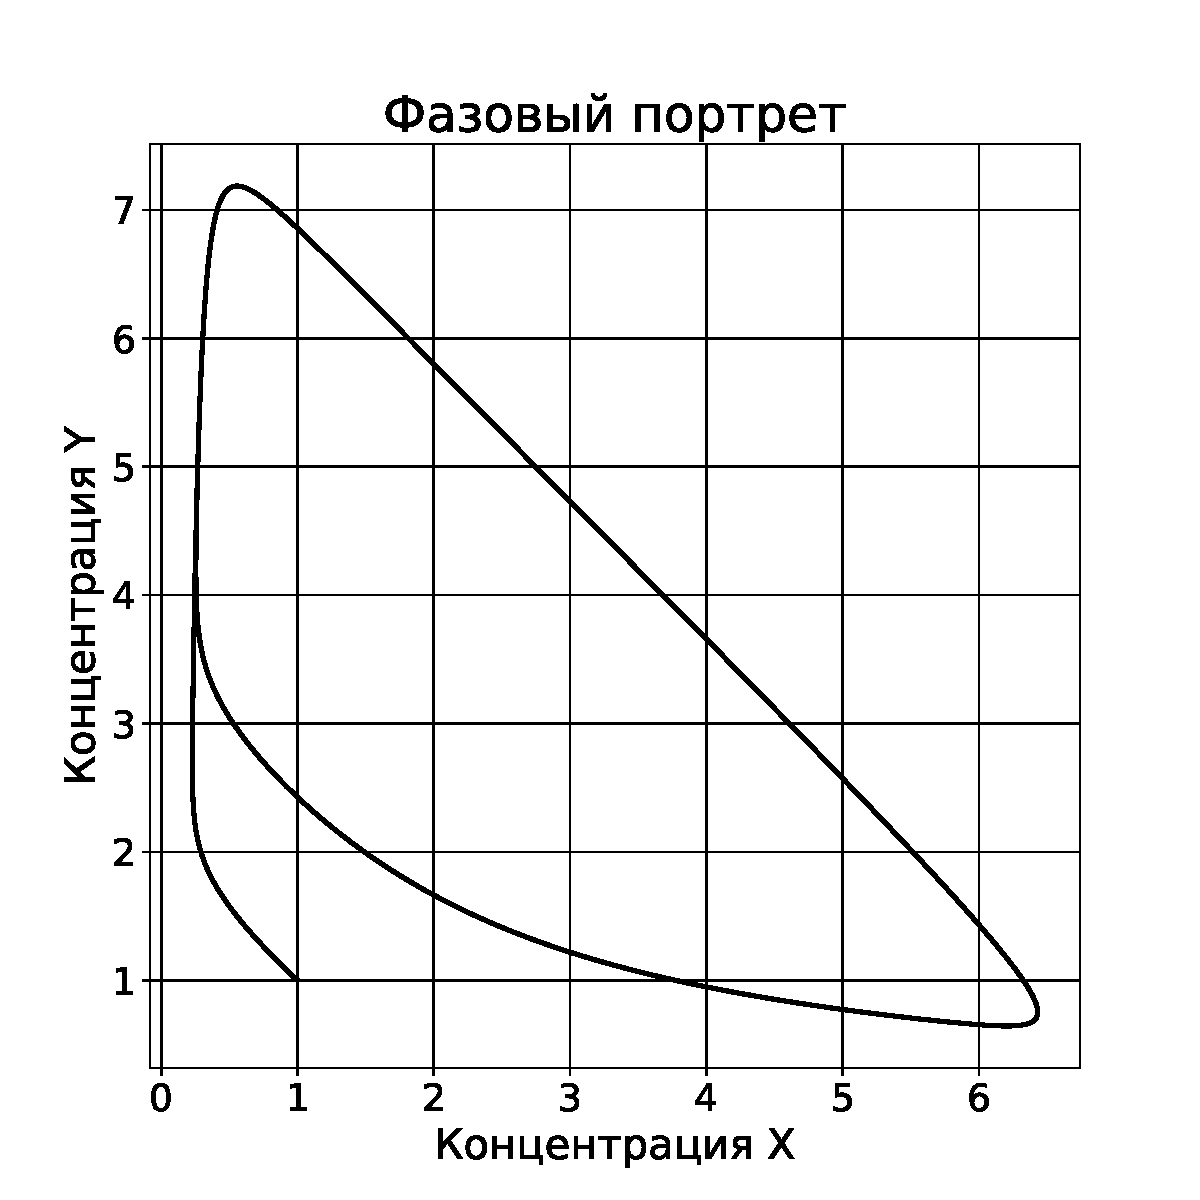
\includegraphics[width=0.8\linewidth]{Pictures/RungeKutta_B_4.0_phase}}
				\end{minipage}
				\caption{Решение методом Рунге-Кутты 4 порядка}
			\end{figure}
			\fillandplacepagenumber
		\end{landscape}
		
		
		\newpage
		\thispagestyle{empty}
		\begin{landscape}
			\begin{figure}[h!]
				\begin{minipage}[h]{0.55\linewidth}
					\center{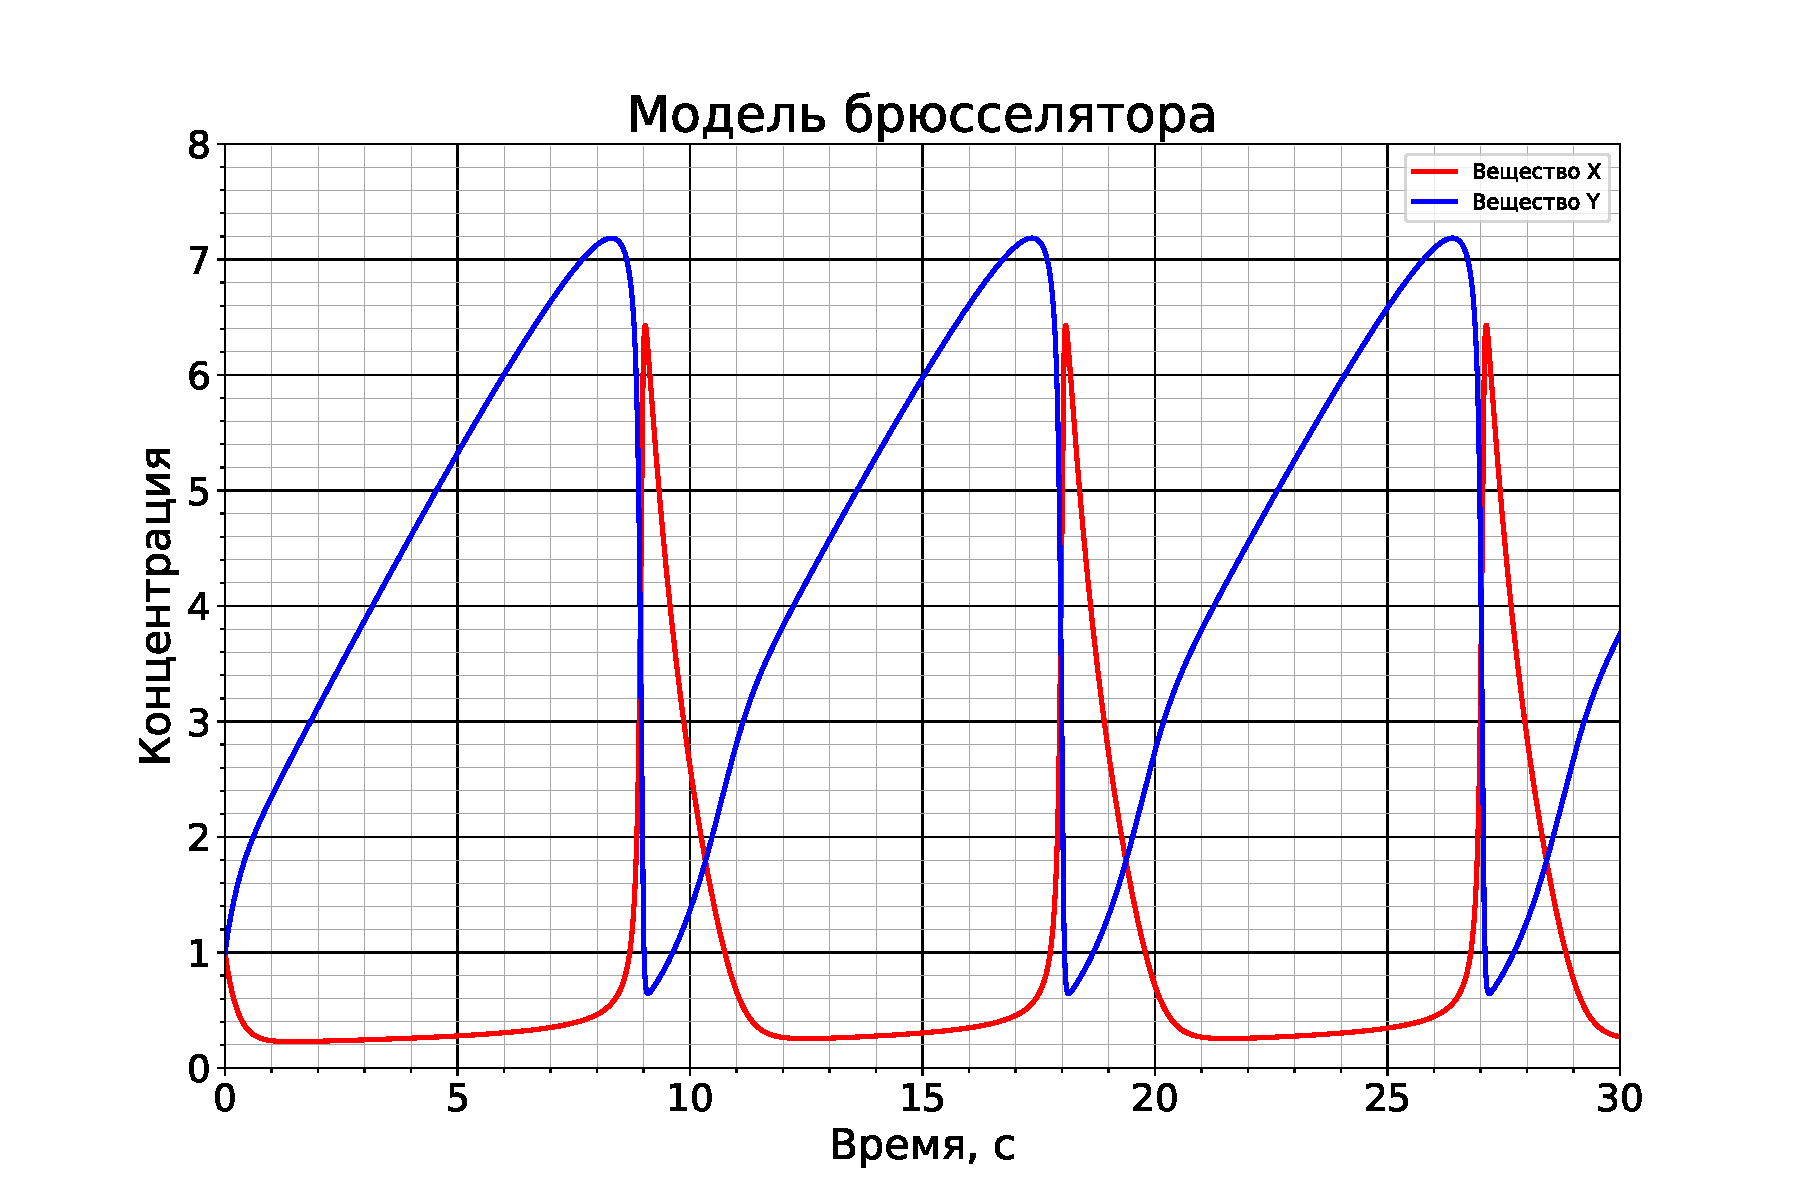
\includegraphics[width=1.2\linewidth]{Pictures/Adams_B_4.0_conc}}
				\end{minipage}
				\hfill
				\begin{minipage}[h]{0.55\linewidth}
					\center{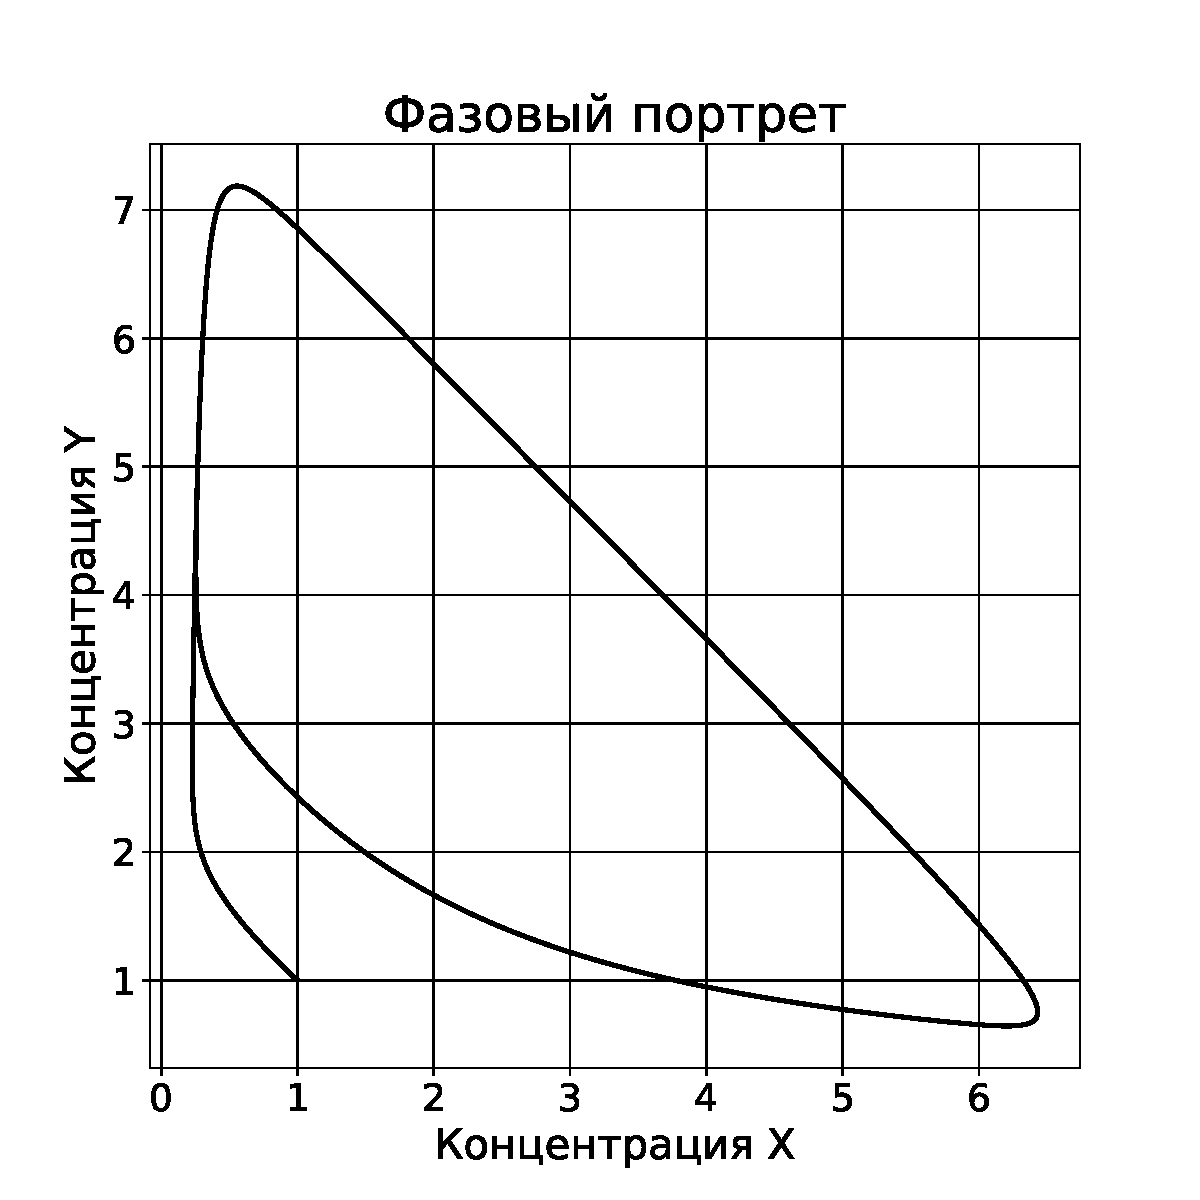
\includegraphics[width=0.8\linewidth]{Pictures/Adams_B_4.0_phase}}
				\end{minipage}
				\caption{Решение методом Адамса 4 порядка}
			\end{figure}
			\fillandplacepagenumber
		\end{landscape}
	
	
		\newpage
		\thispagestyle{empty}
		\begin{landscape}
			\textbf{5)} $A = 1$, $B = 5$	
			\begin{figure}[h!]
				\begin{minipage}[h]{0.55\linewidth}
					\center{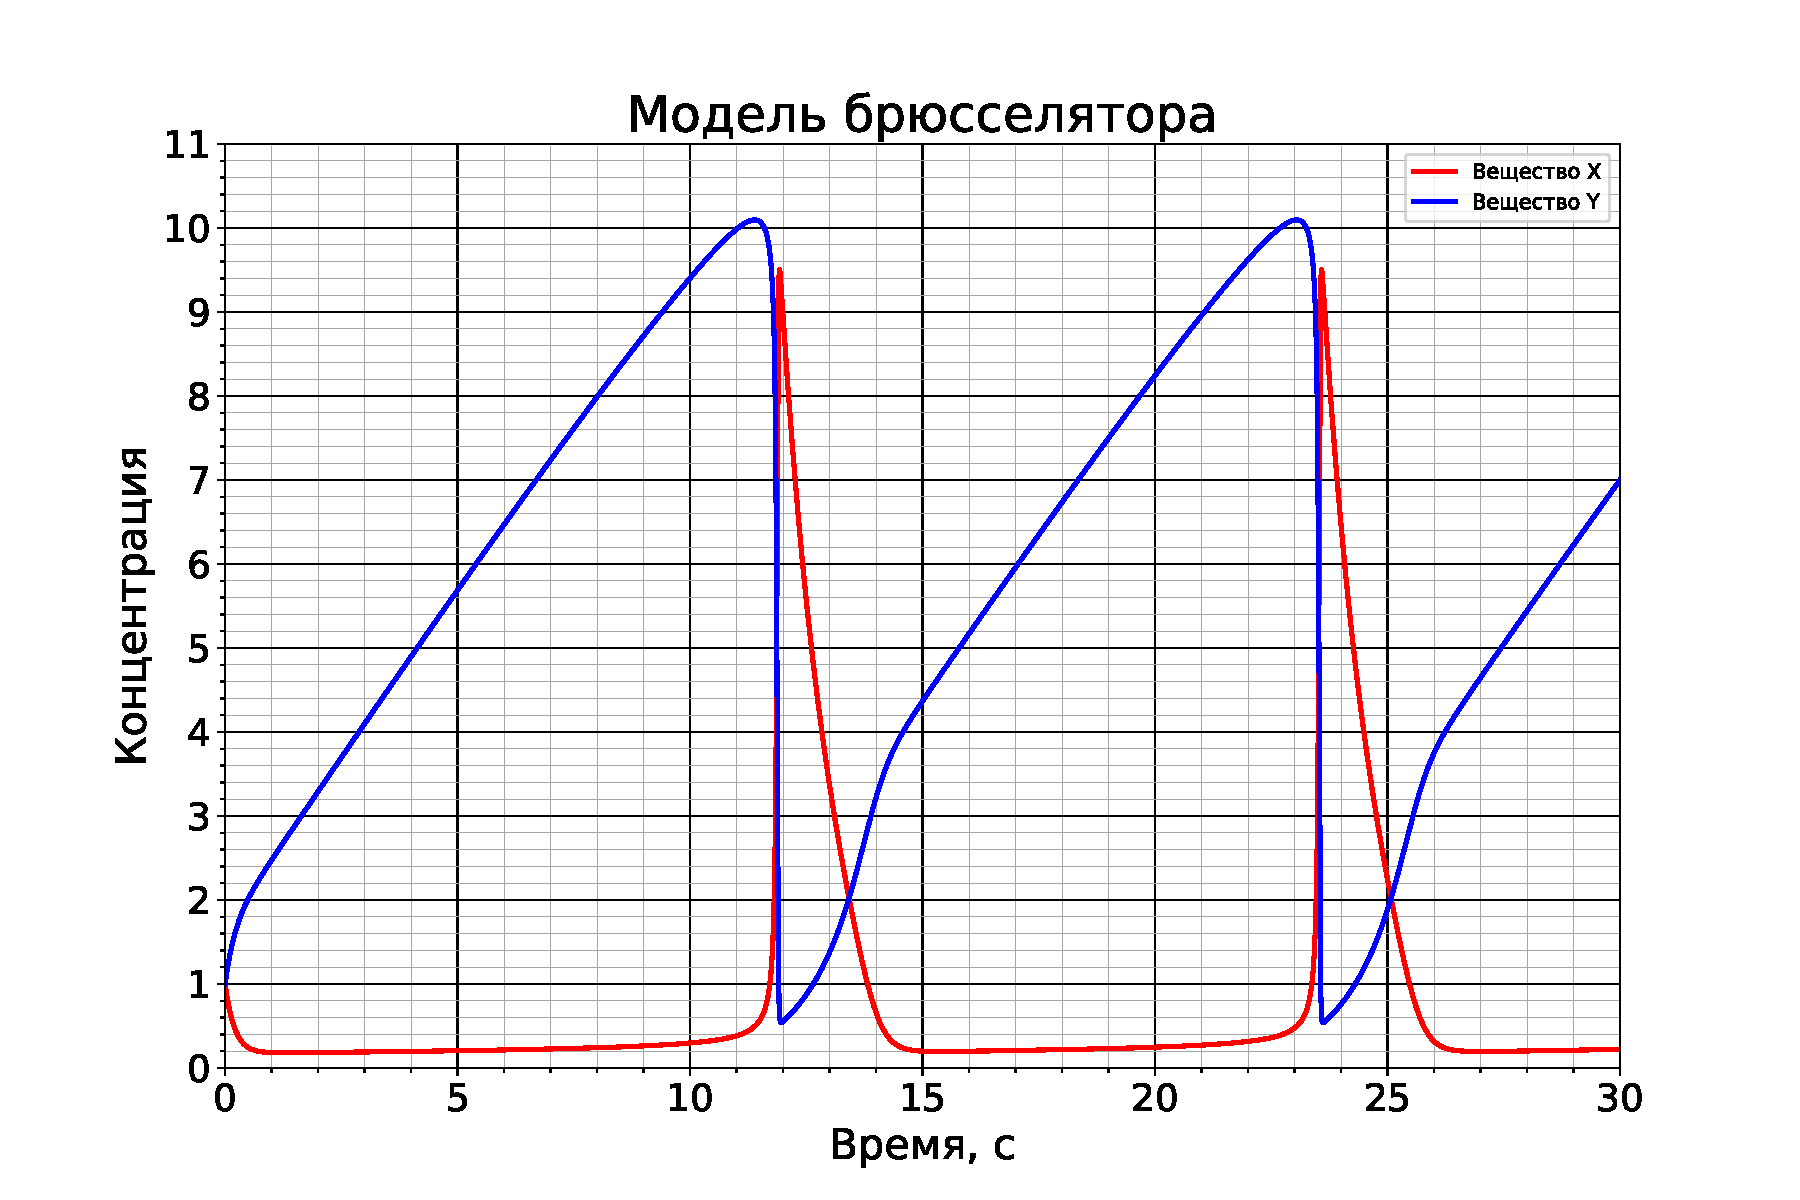
\includegraphics[width=1.2\linewidth]{Pictures/RungeKutta_B_5.0_conc}}
				\end{minipage}
				\hfill
				\begin{minipage}[h]{0.55\linewidth}
					\center{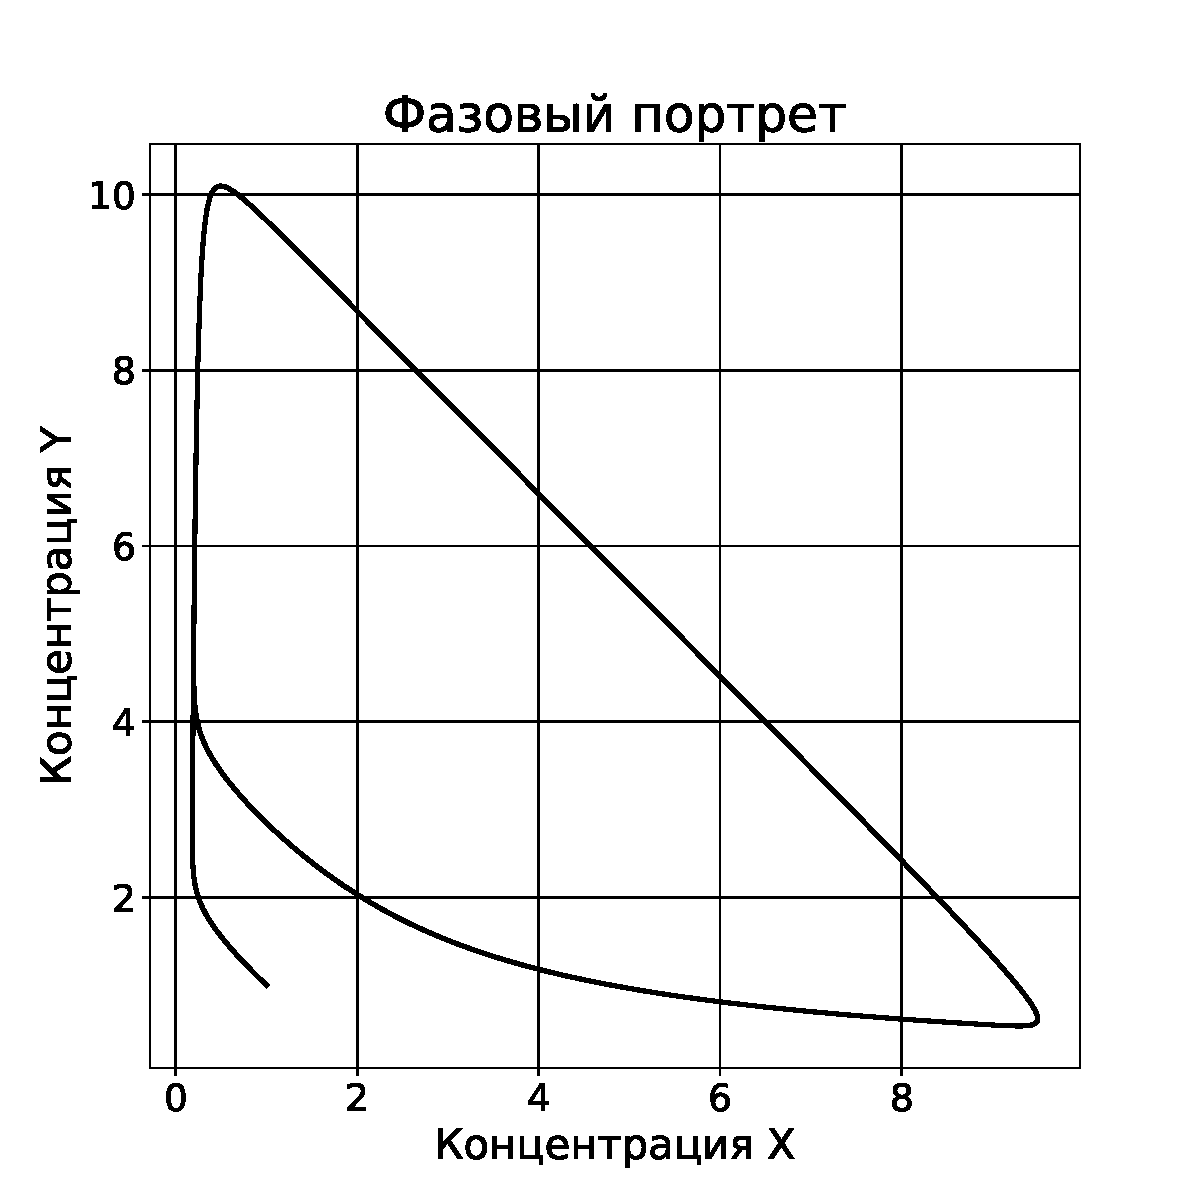
\includegraphics[width=0.8\linewidth]{Pictures/RungeKutta_B_5.0_phase}}
				\end{minipage}
				\caption{Решение методом Рунге-Кутты 4 порядка}
			\end{figure}
			\fillandplacepagenumber
		\end{landscape}
		
		
		\newpage
		\thispagestyle{empty}
		\begin{landscape}
			\begin{figure}[h!]
				\begin{minipage}[h]{0.55\linewidth}
					\center{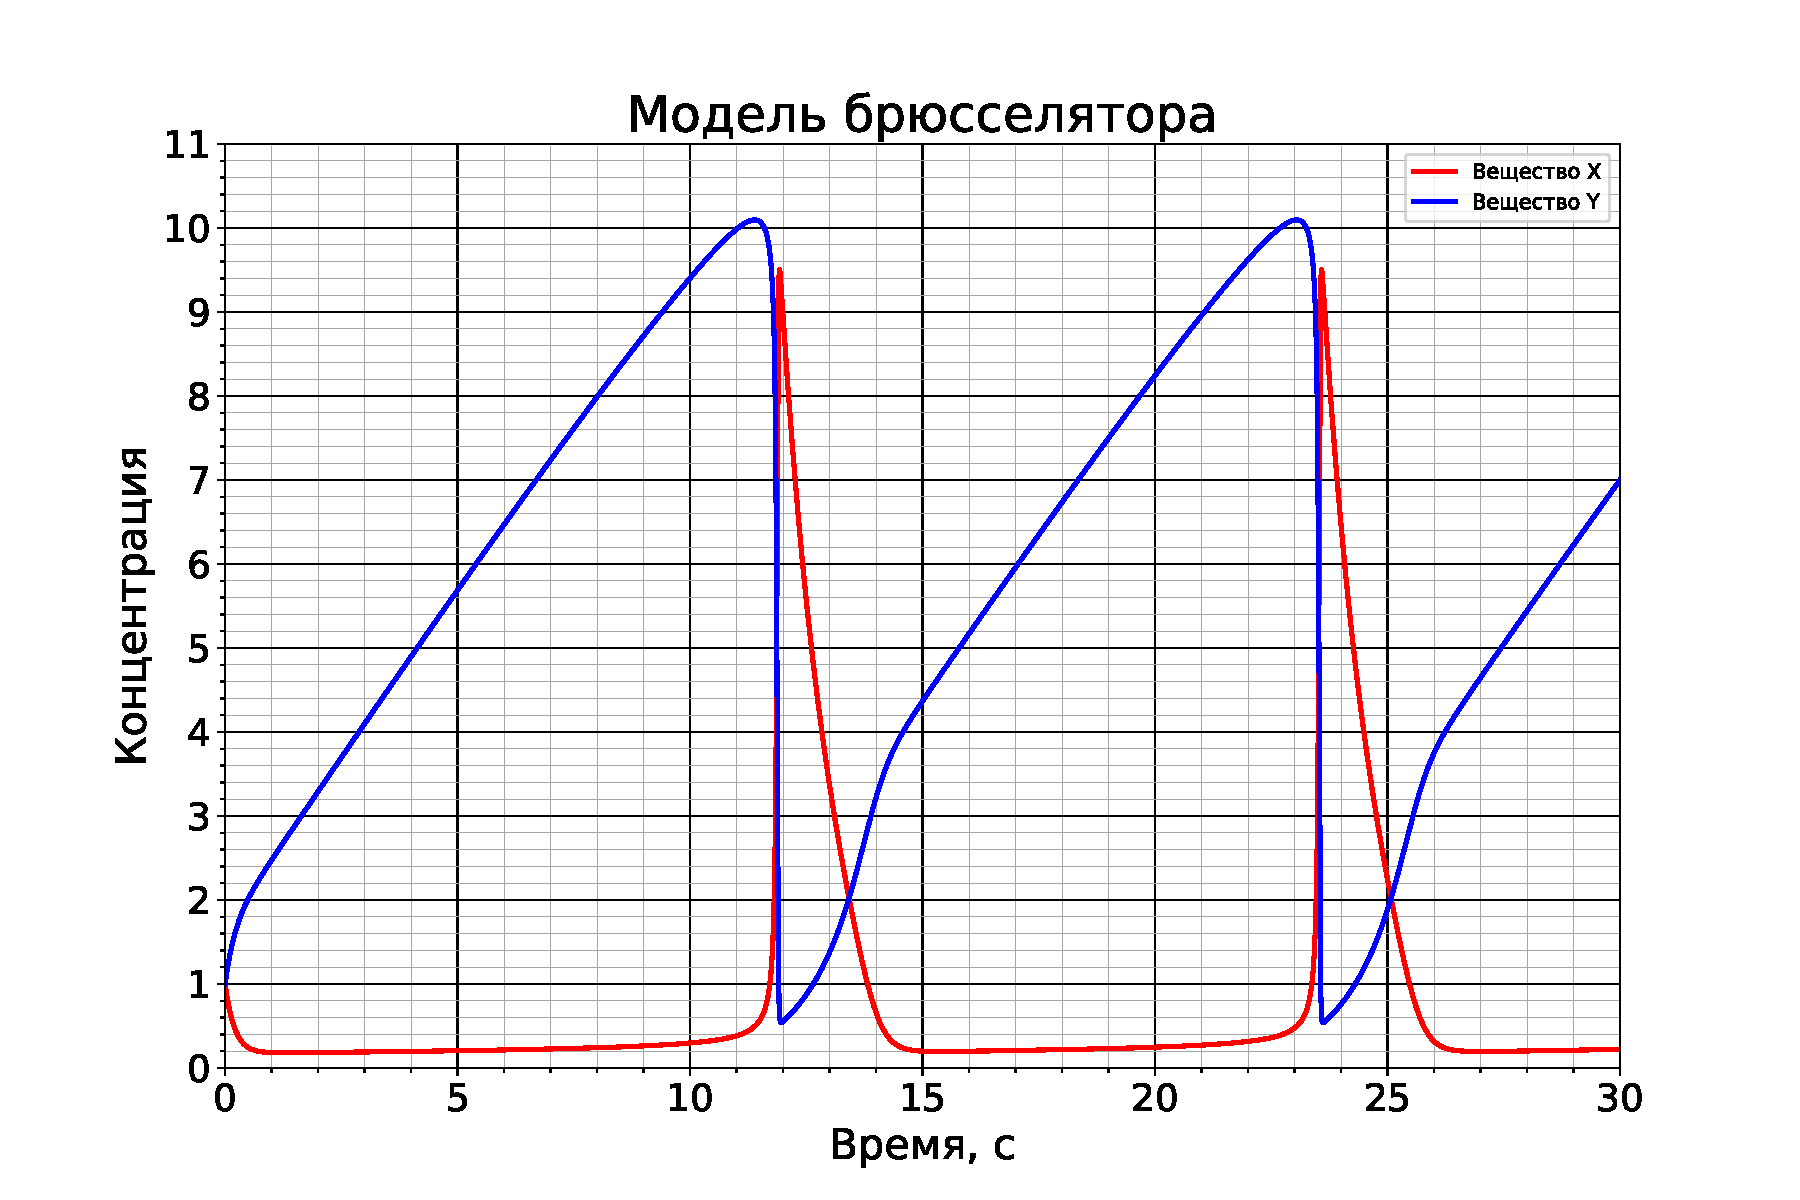
\includegraphics[width=1.2\linewidth]{Pictures/Adams_B_5.0_conc}}
				\end{minipage}
				\hfill
				\begin{minipage}[h]{0.55\linewidth}
					\center{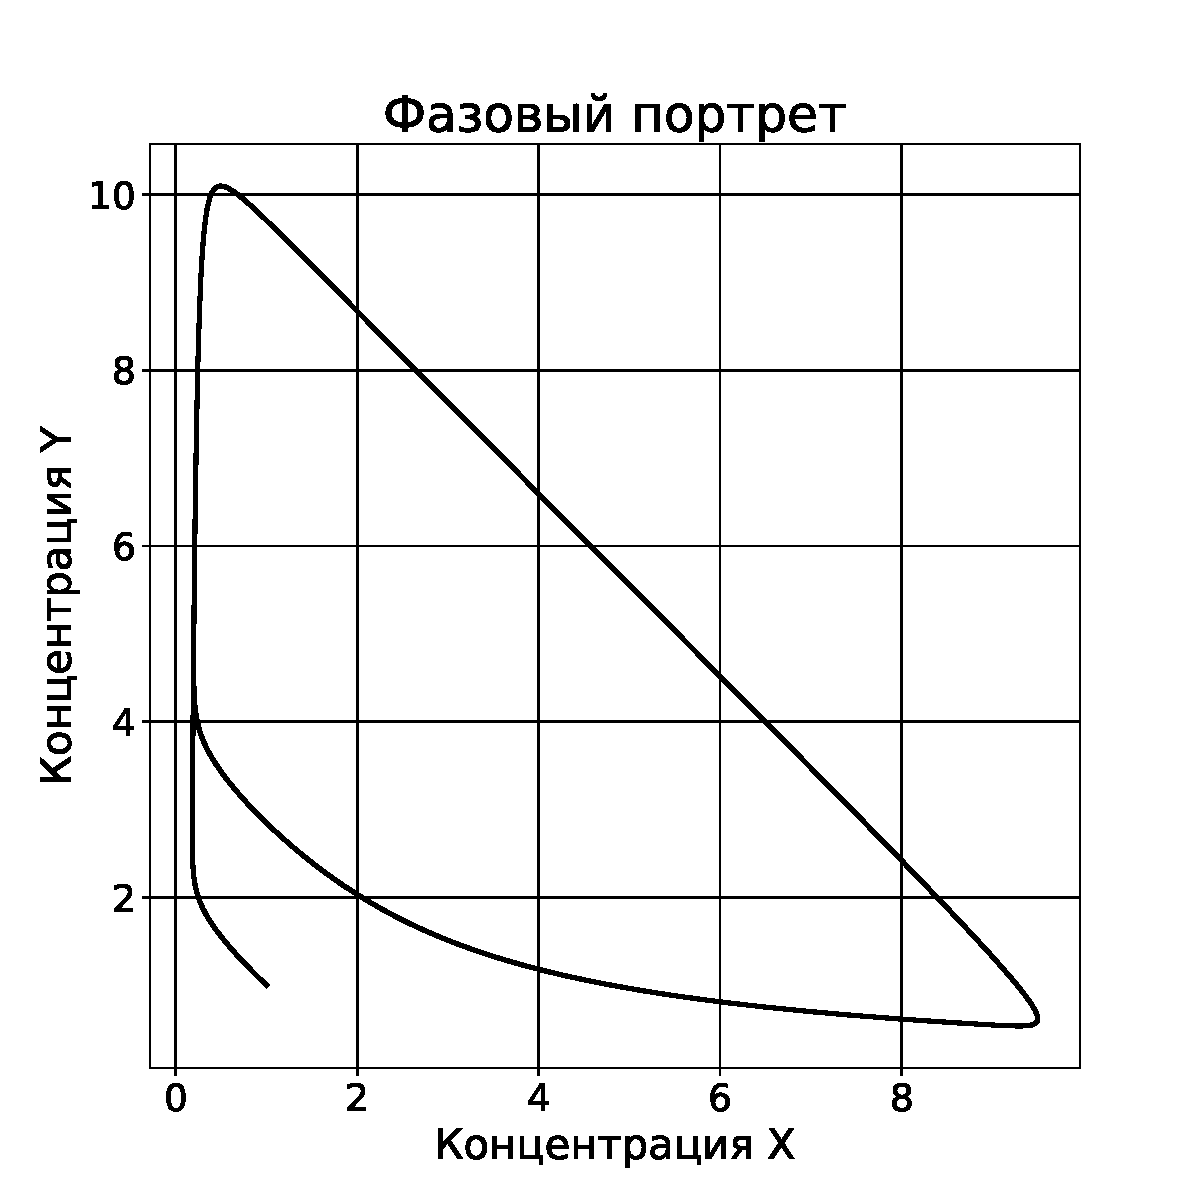
\includegraphics[width=0.8\linewidth]{Pictures/Adams_B_5.0_phase}}
				\end{minipage}
				\caption{Решение методом Адамса 4 порядка}
			\end{figure}
			\fillandplacepagenumber
		\end{landscape}
	
		
		\restoregeometry
		\newpage
		Как видим, результаты, даваемые обоими методами, совпадают. Также мы можем отчетливо увидеть предельный цикл на фазовом портрете.
	
		\tocsection{Вывод}
		В данной работе мы рассмотрели и реализовали методы численного решения систем ОДУ. А именного классический метод Рунге-Кутты 4 порядка и многошаговый метод Адамса 4 порядка. Решения, полученные этими способами, совпадают.
		
		
\end{document}